\documentclass[a4paper, 10pt]{article}

\usepackage[margin = 1in]{geometry} % for spacing around
\usepackage{graphicx} % for including images in your pdfs
\usepackage{xcolor} % for including colors in your pdf
\usepackage{soul} % for text decoration
\usepackage[utf8]{inputenc} % for encoded text
\usepackage[T1]{fontenc}
\usepackage{setspace} % for setting different line spacings between paragrafs.
\usepackage{enumerate} % for letting us get more detailed enumerate lists
\usepackage{multirow} % to let us combine more rows together
\usepackage{colortbl} % for decorating tables
\usepackage{amsmath} % used for representing more complicated math displays
\usepackage{supertabular}
\usepackage{longtable} % both of these packages are used to making really big tables
\usepackage{wrapfig} % allows us to wrap text around figures
\usepackage{fancyhdr} % for making fancy headers
%\usepackage{bibtex} % for making better bibliographies
\usepackage[pdftex]{hyperref} % for letting us make links
\usepackage{lscape} % Allows us to flip from portrait to landspace
\usepackage{tikz} % for high detailed drawing
\usepackage{multicol} % To put things side by side
\usepackage{rotating} % For rotating objects
% \usepackage{draftwatermark} % For adding watermarks
\usepackage{MnSymbol} % for using multiple symbols
\usepackage{mathtools} % Used for more math symbols
\usepackage{xfrac} % For more complciated fractions and to add derivitives
\usepackage{hyperref} % for hyper links
\usepackage{enumitem} % for better enum lists
\usepackage{tcolorbox} % for adding colored text boxes
\usepackage{bm} % Adding bold text to math inputs
\usepackage{pgfplots} % Used for plotting functions
\pgfplotsset{compat=1.18}
\usepackage[siunitx]{circuitikz} % For drawing circuits
\usepackage{caption} % For adding captions to images
\usepackage{siunitx} % Add this line to import the siunitx package
\usepackage{booktabs} % For prettier tables
\usepackage{subcaption} % For subfigures

% Setting up the default image path
\graphicspath{{../../global-assets/images/}}

% Implementing authro details
\title{Lab Report number I - Title of the lab report\\
	ENS203 - Electrical Circuits I}
\author{Emre Arapcic-Uevak\\220302289}
\date{}

% Setting up the fancy page style
\fancypagestyle{customStyle}{
	\lhead{} \chead{} \rhead{}
	\lfoot{} \cfoot{\thepage} \rfoot{}
	\renewcommand{\headrulewidth}{0pt}
	\renewcommand{\footrulewidth}{1pt}
}
\pagestyle{customStyle}

% Custom commands


\begin{document}
	\begin{titlepage}
		\begin{center}
			\vspace*{\stretch{1}} % Add vertical space before the title

			{\Large\bfseries Lab Report number 3 \\[0.5em] Series / Parallel Circuits\par}
			\vspace{1cm} % Space between title and course title

			{\large ENS203 – Electrical Circuits I\par}
			\vspace{1cm} % Space between course title and your name/ID

			{\large Emre Arapcic-Uevak \\ 220302289\par}
			\vspace{.3cm} % Space between your name/ID and assistant name
			{\large Afan Haznadarevic \\ 220302128\par}
			\vspace{1cm} % Space between your name/ID and assistant name

			{\large Assistant: Adil Hasanbasic\par}
			\vspace{\stretch{2}} % Variable vertical space between assistant name and bottom
			
\includegraphics[width=0.5\textwidth]{Logo.png}
			\vspace{5mm}
			
			\textsc{\LARGE Internation University of Sarajevo}\\[1.5cm]
			\textsc{\Large ENS203 - Electrical Circuits I}\\[0.5cm]
			
			\rule{\linewidth}{0.5mm} \\[0.4cm]
			{ \huge \bfseries Lab Report number III - Series / Parallel Circuits}\\[0.4cm]
			\rule{\linewidth}{0.5mm} \\[1.5cm]
			
			\vfill
			
			% Bottom of the page
			{\large \today}
		\end{center}
	\end{titlepage}
	\pagebreak

	\tableofcontents
	\pagebreak
	
	\listoffigures
	\pagebreak
	
	\section{Objective}
		The objective of this lab is to understand Kirchhoff's laws and how they can be applied to series and parallel circuits.
		We will build three different circuits in this lab and try to show the validity of Kirchhoff's laws.
		
		\subsection{Kirchhoff's Laws}
			\begin{itemize}
				\item Kirchhoff's Current Law (KCL): The sum of currents entering a node is equal to the sum of currents leaving the node.
				\item Kirchhoff's Voltage Law (KVL): The sum of voltages around a closed loop is equal to zero.
			\end{itemize}
	
		\subsection{Equipment}
			\begin{itemize}
				\item Breadboard
				\item Resistors 1\si{\kilo\Omega}, 10 \si{\kilo\Omega}, 100 \si{\Omega}
				\item 1 LED
				\item DC Power supply
				\item Multimeter
			\end{itemize}

			\subsubsection{Breadboard}
				A breadboard is a construction base for prototyping of electronics.A breadboard consists of plastic block holding a matrix of electrical sockets of a size suitable for gripping thin connecting wire, 
				component wires or the pins of transistors and integrated circuits (ICs). The sockets are connected inside the board, usually in rows of five sockets.

				\begin{figure}[h!]
					\centering
					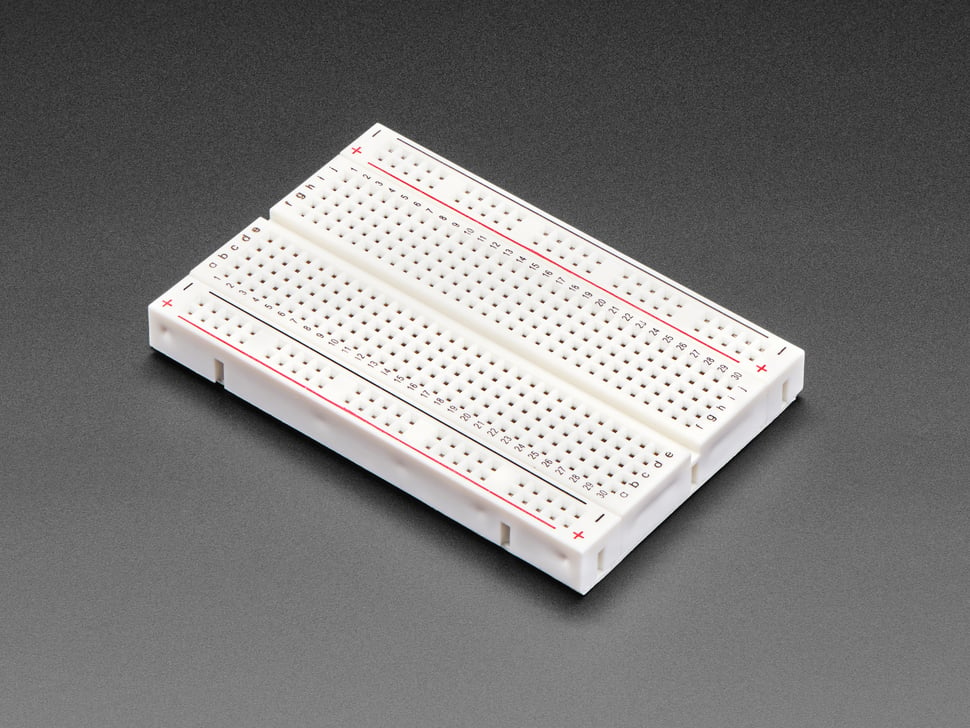
\includegraphics[width=0.5\textwidth]{images/breadboard.jpeg}
					\caption{A breadboard}
					\label{fig:breadboard}
				\end{figure}
			

			\pagebreak

			\subsubsection{Resistors}
				As stated before we needed 3 resistors for this lab report so we took 3 resistors with the proper colour code values and then we measured them and marked them.

				\begin{figure}[h!]
					\centering
					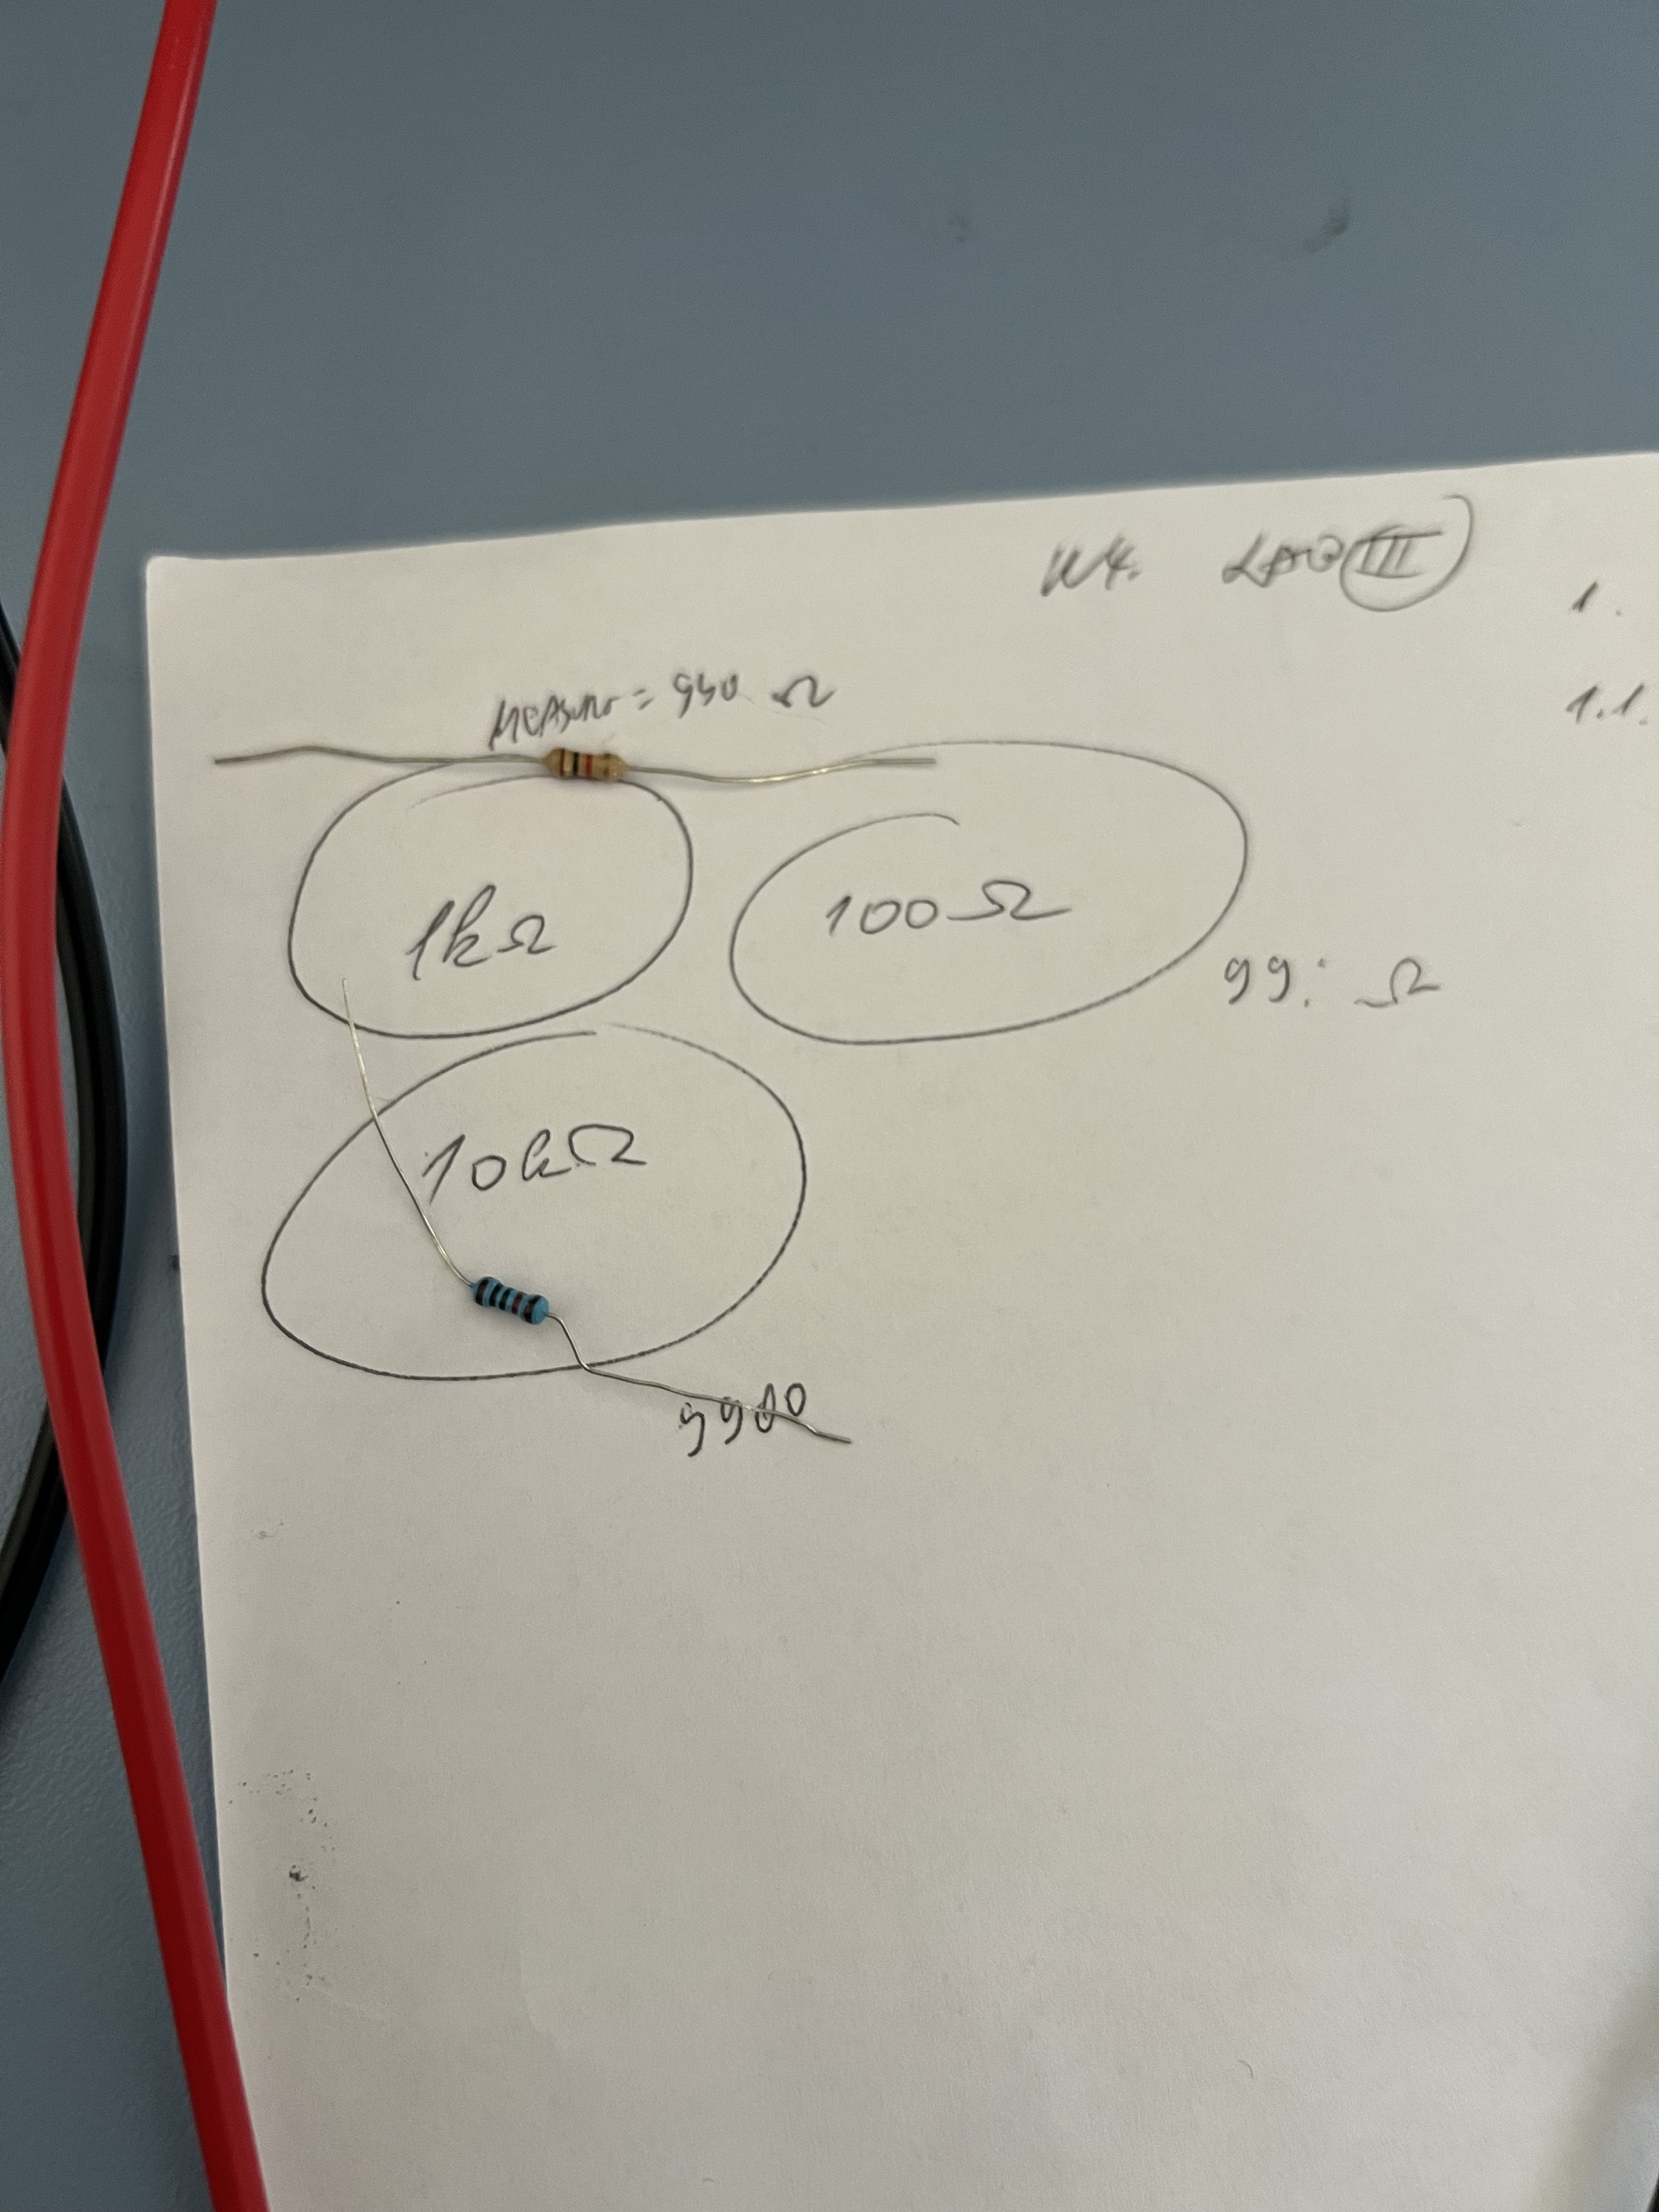
\includegraphics[width=0.35\textwidth]{images/Resistors.jpeg}
					\caption{Resistors with their measured values}
					\label{fig:resistors}
				\end{figure}

	
				\begin{table}[h!]
					\centering
					\begin{tabular}{@{}l|S|S@{}} % l for left, S for siunitx number column
						\toprule
						{Resistor} & {Expected Value (\si{\ohm})} & {Measured Value (\si{\ohm})} \\
						\midrule
						R1 & 100 & 99 \\
						R2 & 1000 & 990 \\
						R3 & 10000 & 9900 \\
						\bottomrule
					\end{tabular}
					\caption{Expected and Measured Resistance Values}
					\label{tab:resistors}
				\end{table}

			\subsubsection{LED}
				An LED (Light Emitting Diode) is a semiconductor device that emits light when an electric current passes through it. LEDs are commonly used in electronic circuits for various purposes, such as indicator lights, displays, and illumination.
				In this lab, a red LED was used. Red LEDs emit red light with a specific wavelength. They are widely used in applications such as traffic lights, electronic displays, and decorative lighting.
				Here is an image of a red LED:

				\begin{figure}[h!]
					\centering
					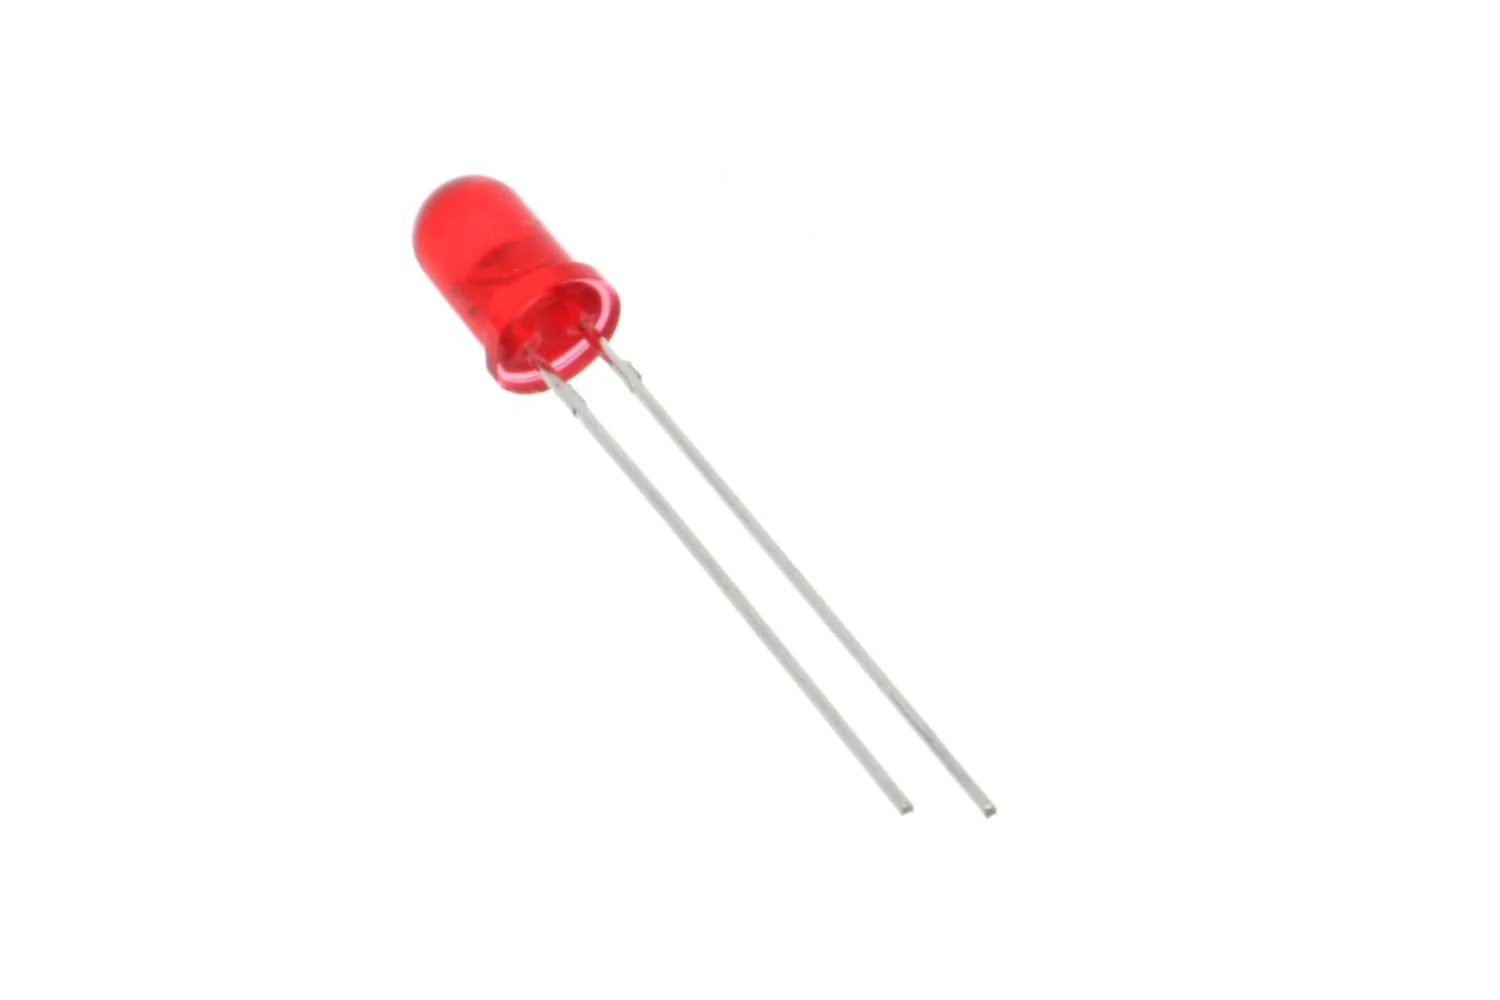
\includegraphics[width = 0.5\textwidth]{images/LED.jpeg}
					\caption{Red LED}
					\label{fig:red_led}
				\end{figure}

			\pagebreak

			\subsubsection{Multimeter}
				The multimeter is a versatile tool used for measuring various electrical quantities. In this lab, we will use it to measure the voltage drops across components, the currents through branches and components, and the resistance of resistors.
				To measure voltage drops, connect the multimeter in parallel across the component of interest. Set the multimeter to the voltage measurement mode and select an appropriate range.
				To measure currents, connect the multimeter in series with the branch or component. Set the multimeter to the current measurement mode and select an appropriate range.
				To measure resistance, disconnect the resistor from the circuit. Connect the multimeter probes to the resistor terminals. Set the multimeter to the resistance measurement mode and select an appropriate range.

				\begin{figure}[h!]
					\centering
					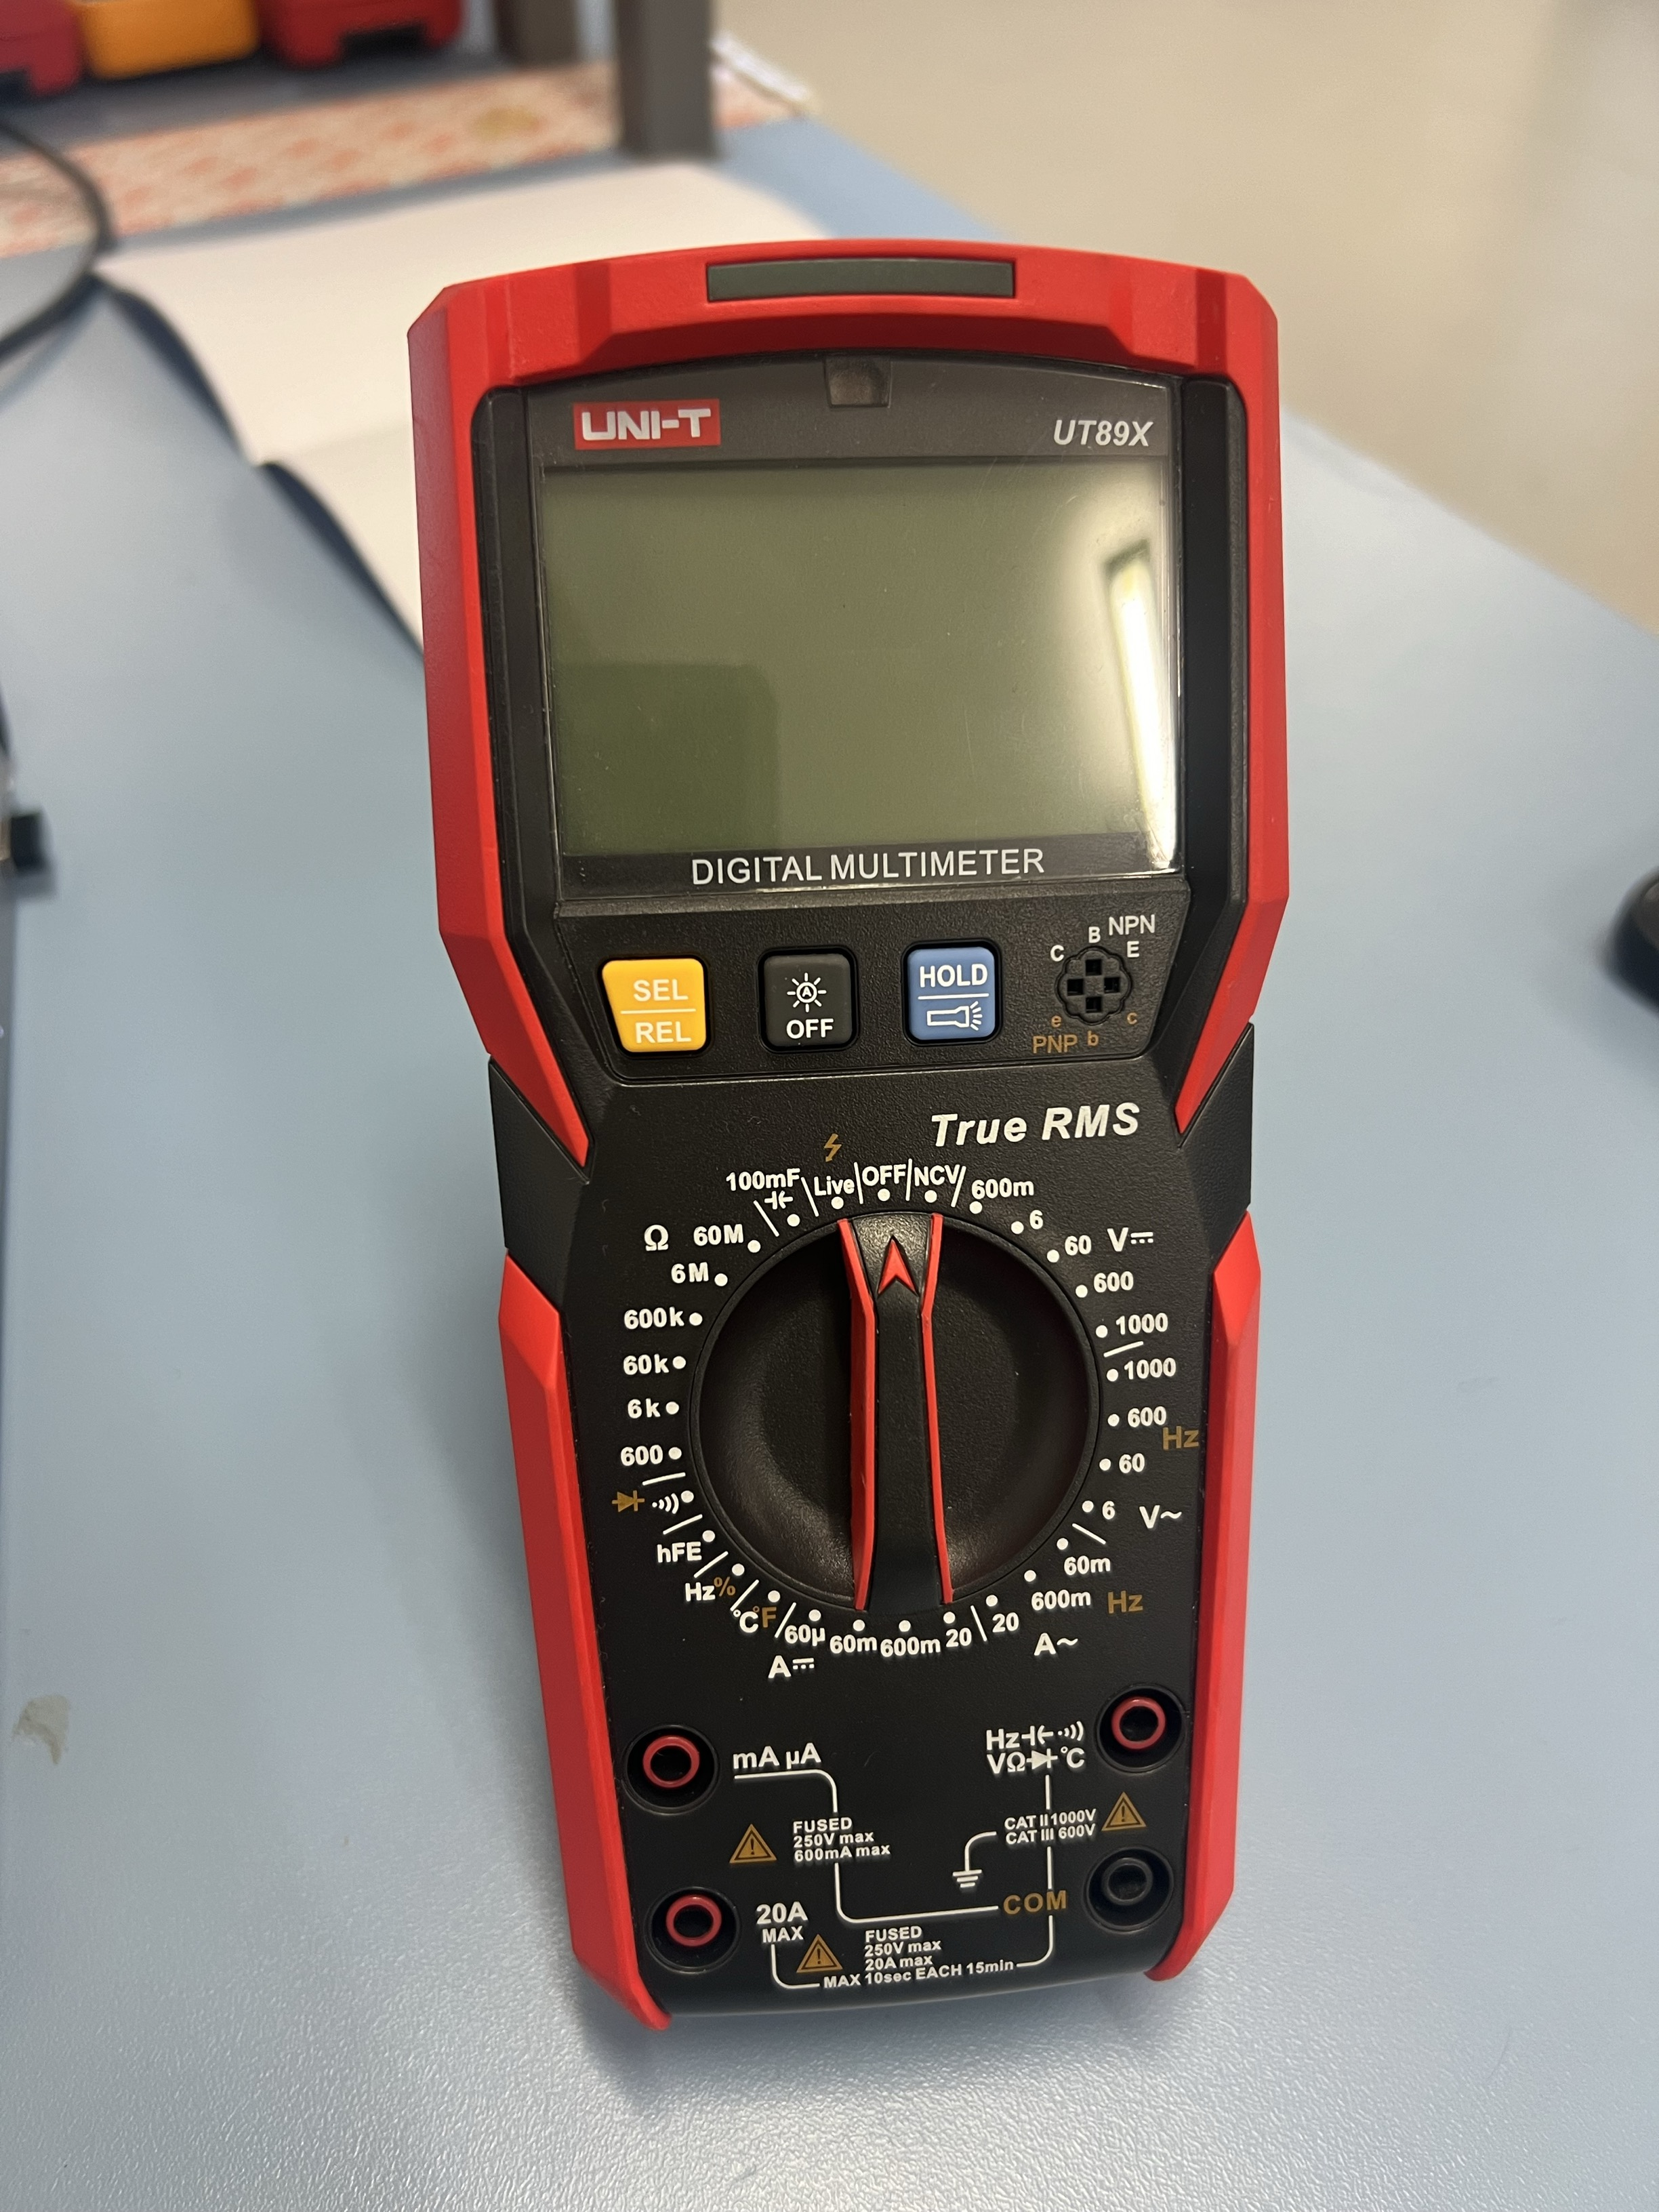
\includegraphics[height = 0.3\textheight]{images/Multimeter.jpeg}
					\caption{Multimeter}
					\label{fig:multi_meter}
				\end{figure}

	\pagebreak
	\section{Circuit 1}
		\begin{figure}[h!]
			\centering
			\begin{circuitikz}[line width=0.75pt]
				\draw
				(0,0) to[V, V=\SI{5}{\volt}, invert, fill=green!50] ++(0,3) % Voltage source
				to[R, l=\SI{100}{\ohm}, fill=red!50] ++(3,0)              % Resistor
				to[led, fill=red!50] ++(0,-3)                              % LED
				-- (0,0);                                                   % Connection back to the beginning
				% Adding an arrow to emphasize voltage drop across the LED
				\draw[<->, >=stealth, thick, blue] (3.9,2) -- node[right] {Voltage drop} (3.9,0.95);
			  \end{circuitikz}
			\caption{Simple LED circuit with a 5V power supply and a 100 ohm resistor.}
			\label{fig:simple_led_circuit}
		\end{figure}

		\subsection{Objectives}
			\begin{itemize}
				\item To measure the voltage drop across the LED.
				\item To measure the voltage drop across the resistor.
				\item Ensure that the sum of the voltage drops is equal to the voltage of the power supply, hence validating Kirchhoff's Voltage Law.
				\item Change the voltage source and see what happense to the LED
				\item Change the resistance and see what happense to the LED
			\end{itemize}

		\subsection{Making the circuit}
			This is a pretty simple circuit to make it all we did was to take a resistor and put in on one of the positive pins on the breadboard and then take the LED,
			put it's anode to be on the same column on the breadboard as the resistor it self and it's cathode we connected to the negative probe of the voltage source.
			You can see the above mentioned circuit on Figure \ref{fig:Physical_LED_Circ}
			\begin{figure}[h!]
				\centering
				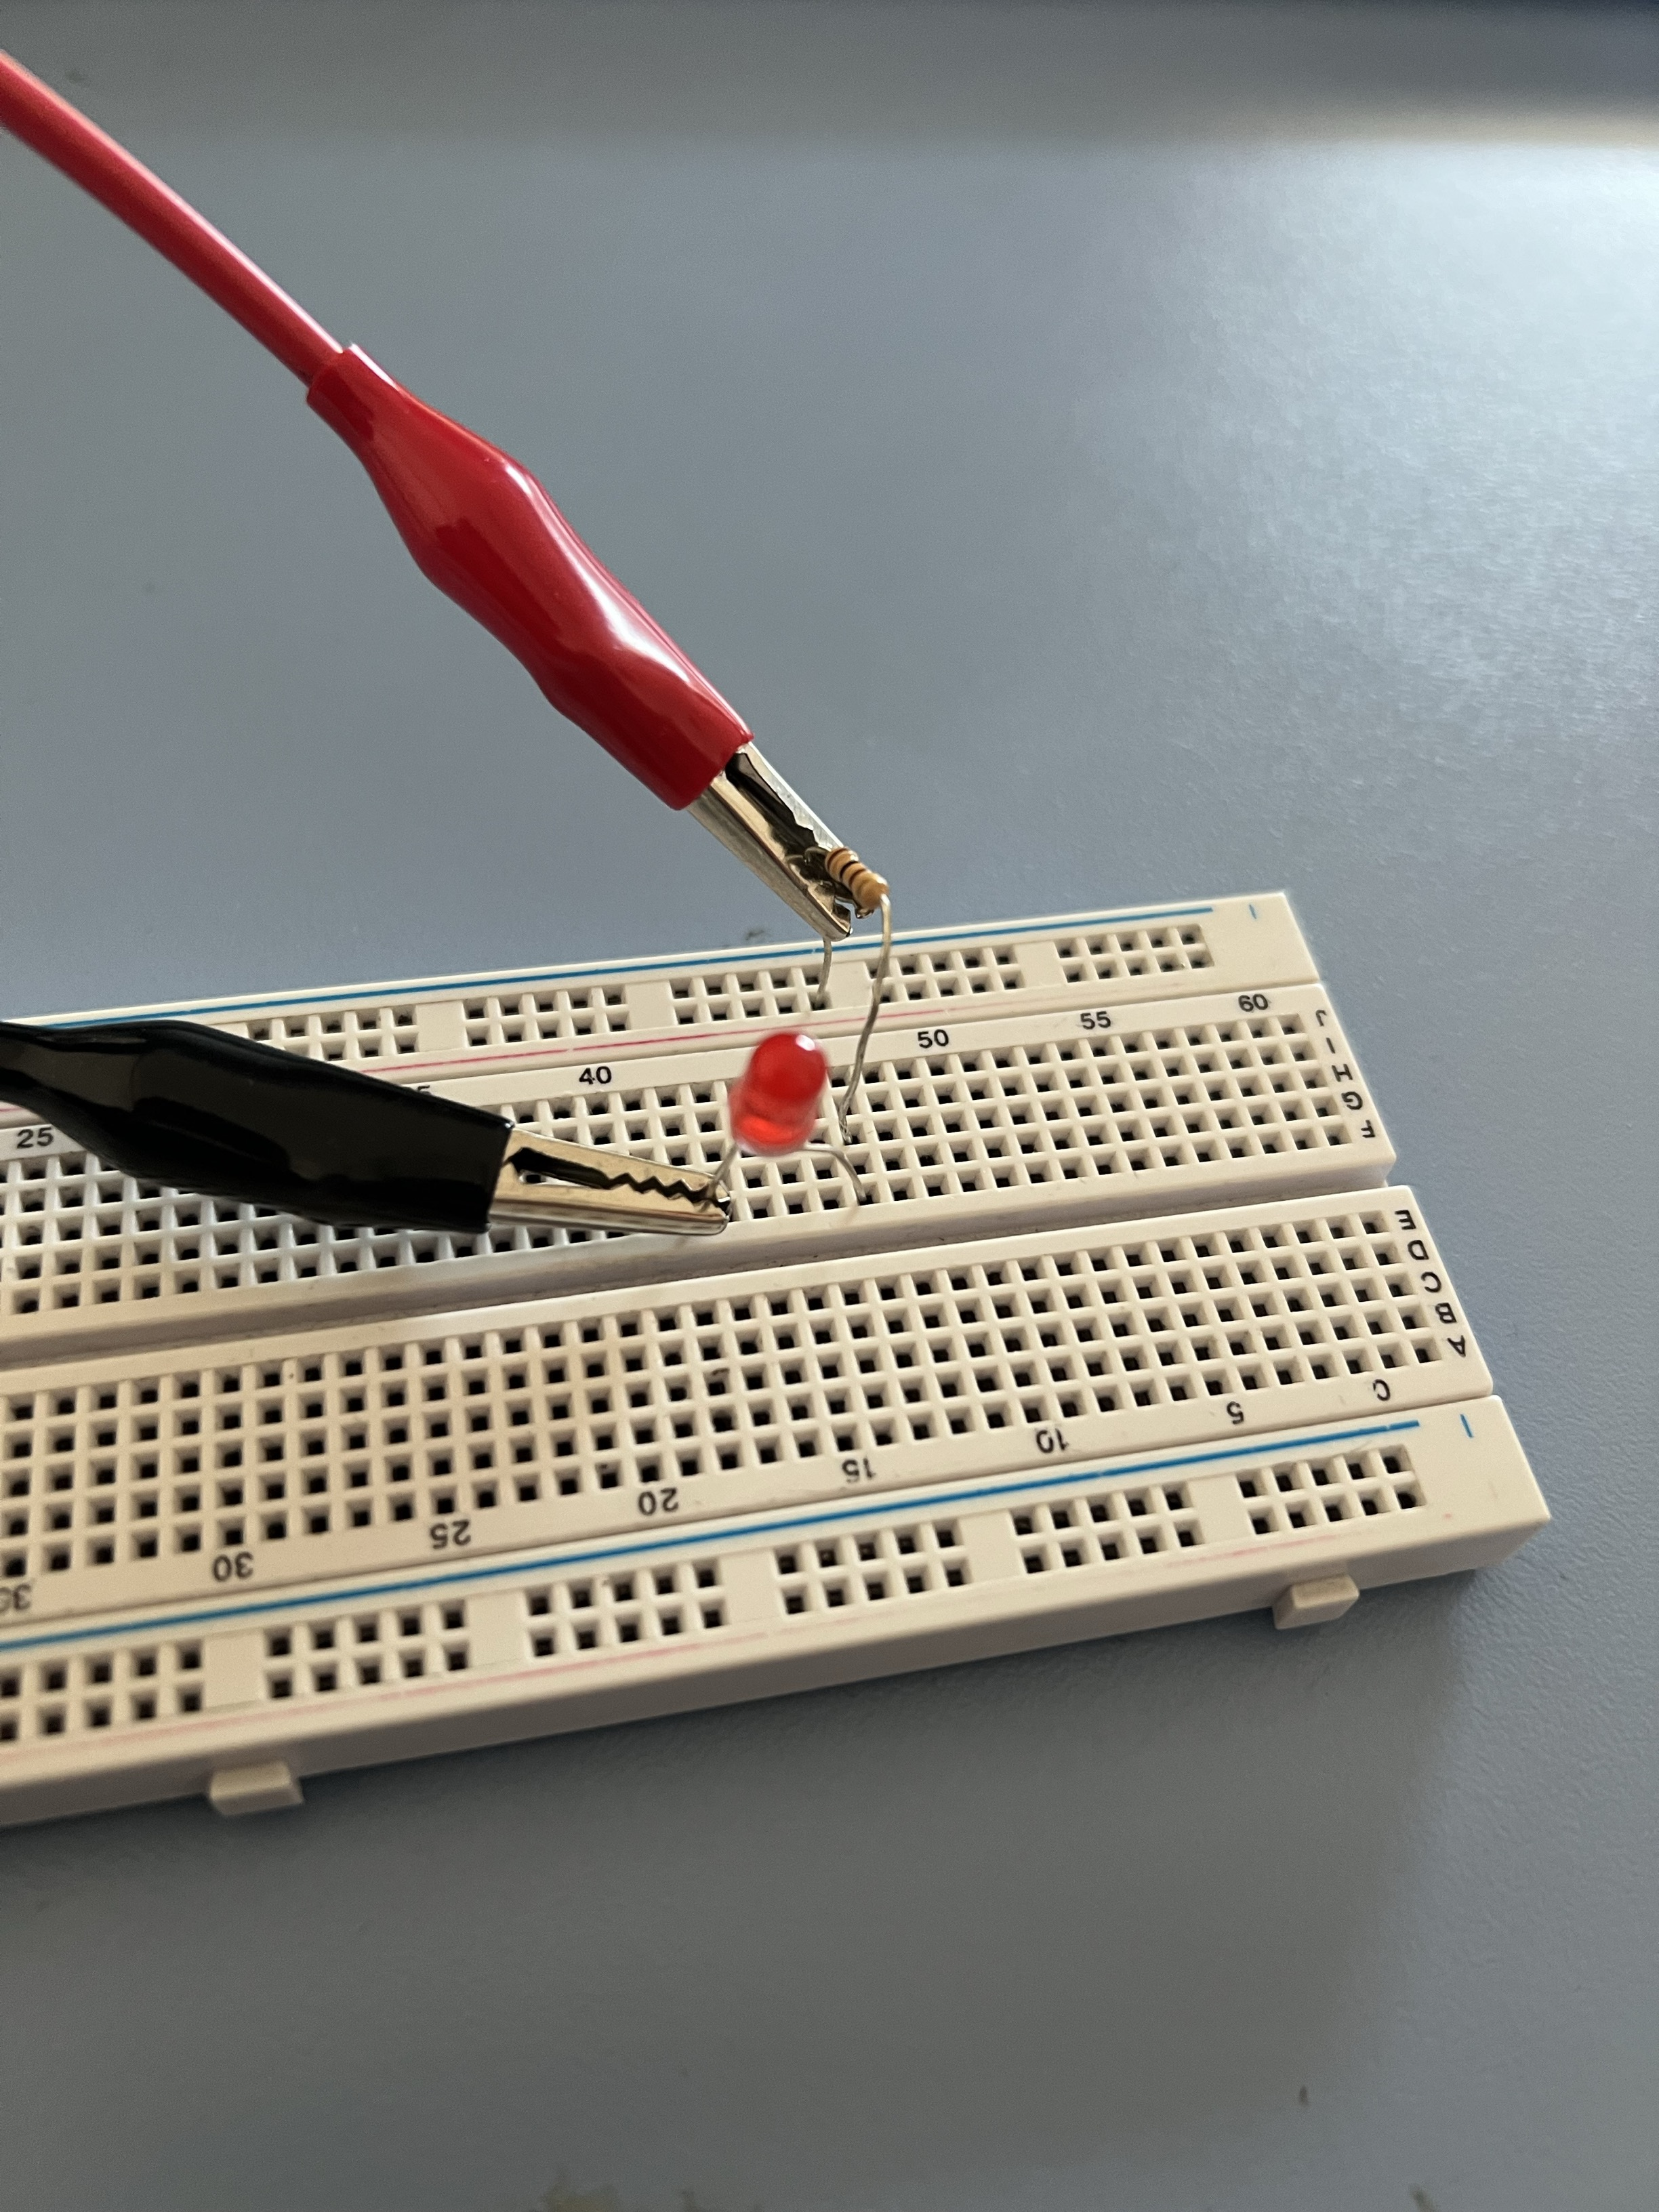
\includegraphics[width = .3\textwidth]{images/Circuit1.jpeg}
				\caption{Simple LED circuit made on the breadboard}
				\label{fig:Physical_LED_Circ}
			\end{figure}
		\pagebreak

		\subsection{Demonstrating \emph{KVL}}
			KVL states that the sum of the voltage drops around a closed loop is equal to zero. 
			In this circuit, we have a single loop, so the sum of the voltage drops across the LED and the resistor should be equal to the voltage of the power supply.
			We measured the voltage drop across the LED and the resistor using a multimeter and compared the sum to the voltage of the power supply.

			
			\begin{figure}[h!]
				\centering
				\begin{subfigure}[b]{0.35\textwidth}
					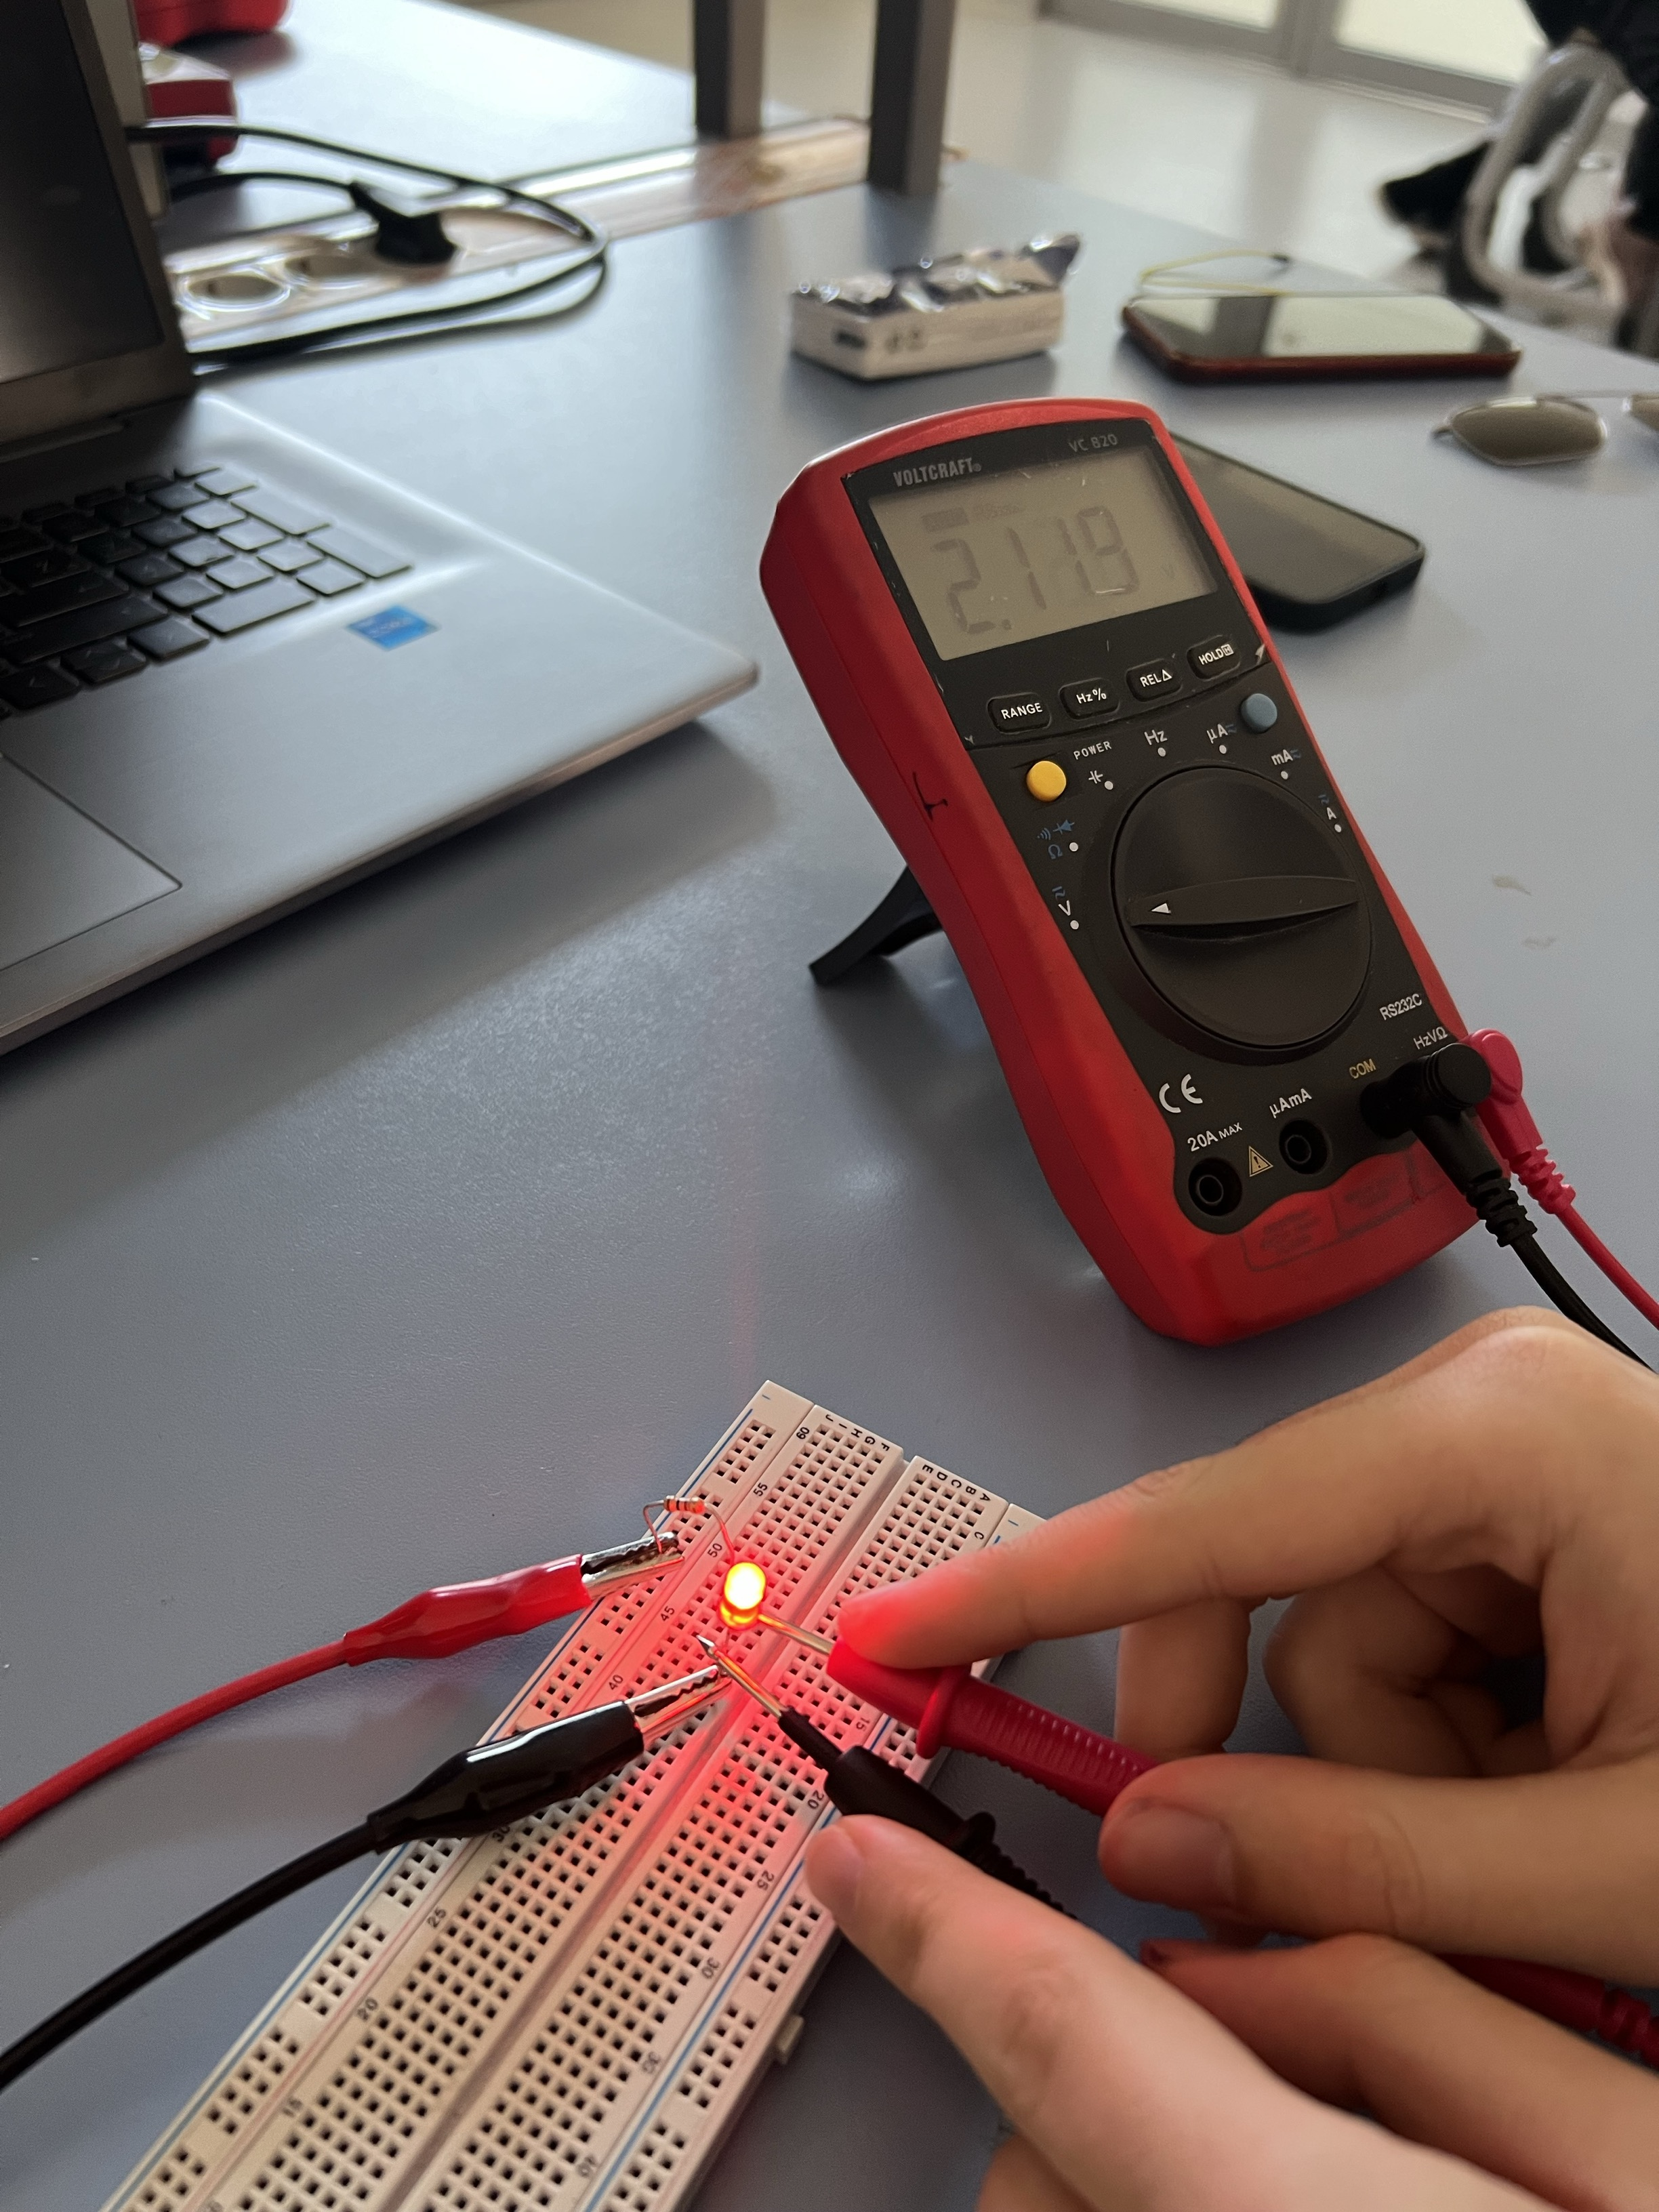
\includegraphics[width=\textwidth]{./images/Circ1_VDrop_LED.jpeg}
					\caption{Voltage drop on the LED}
					\label{sub-fig:VDropLEDCirc1}	
				\end{subfigure}
				\hspace{0.1\textwidth} % This is the gap between the images
				\begin{subfigure}[b]{0.35\textwidth}
					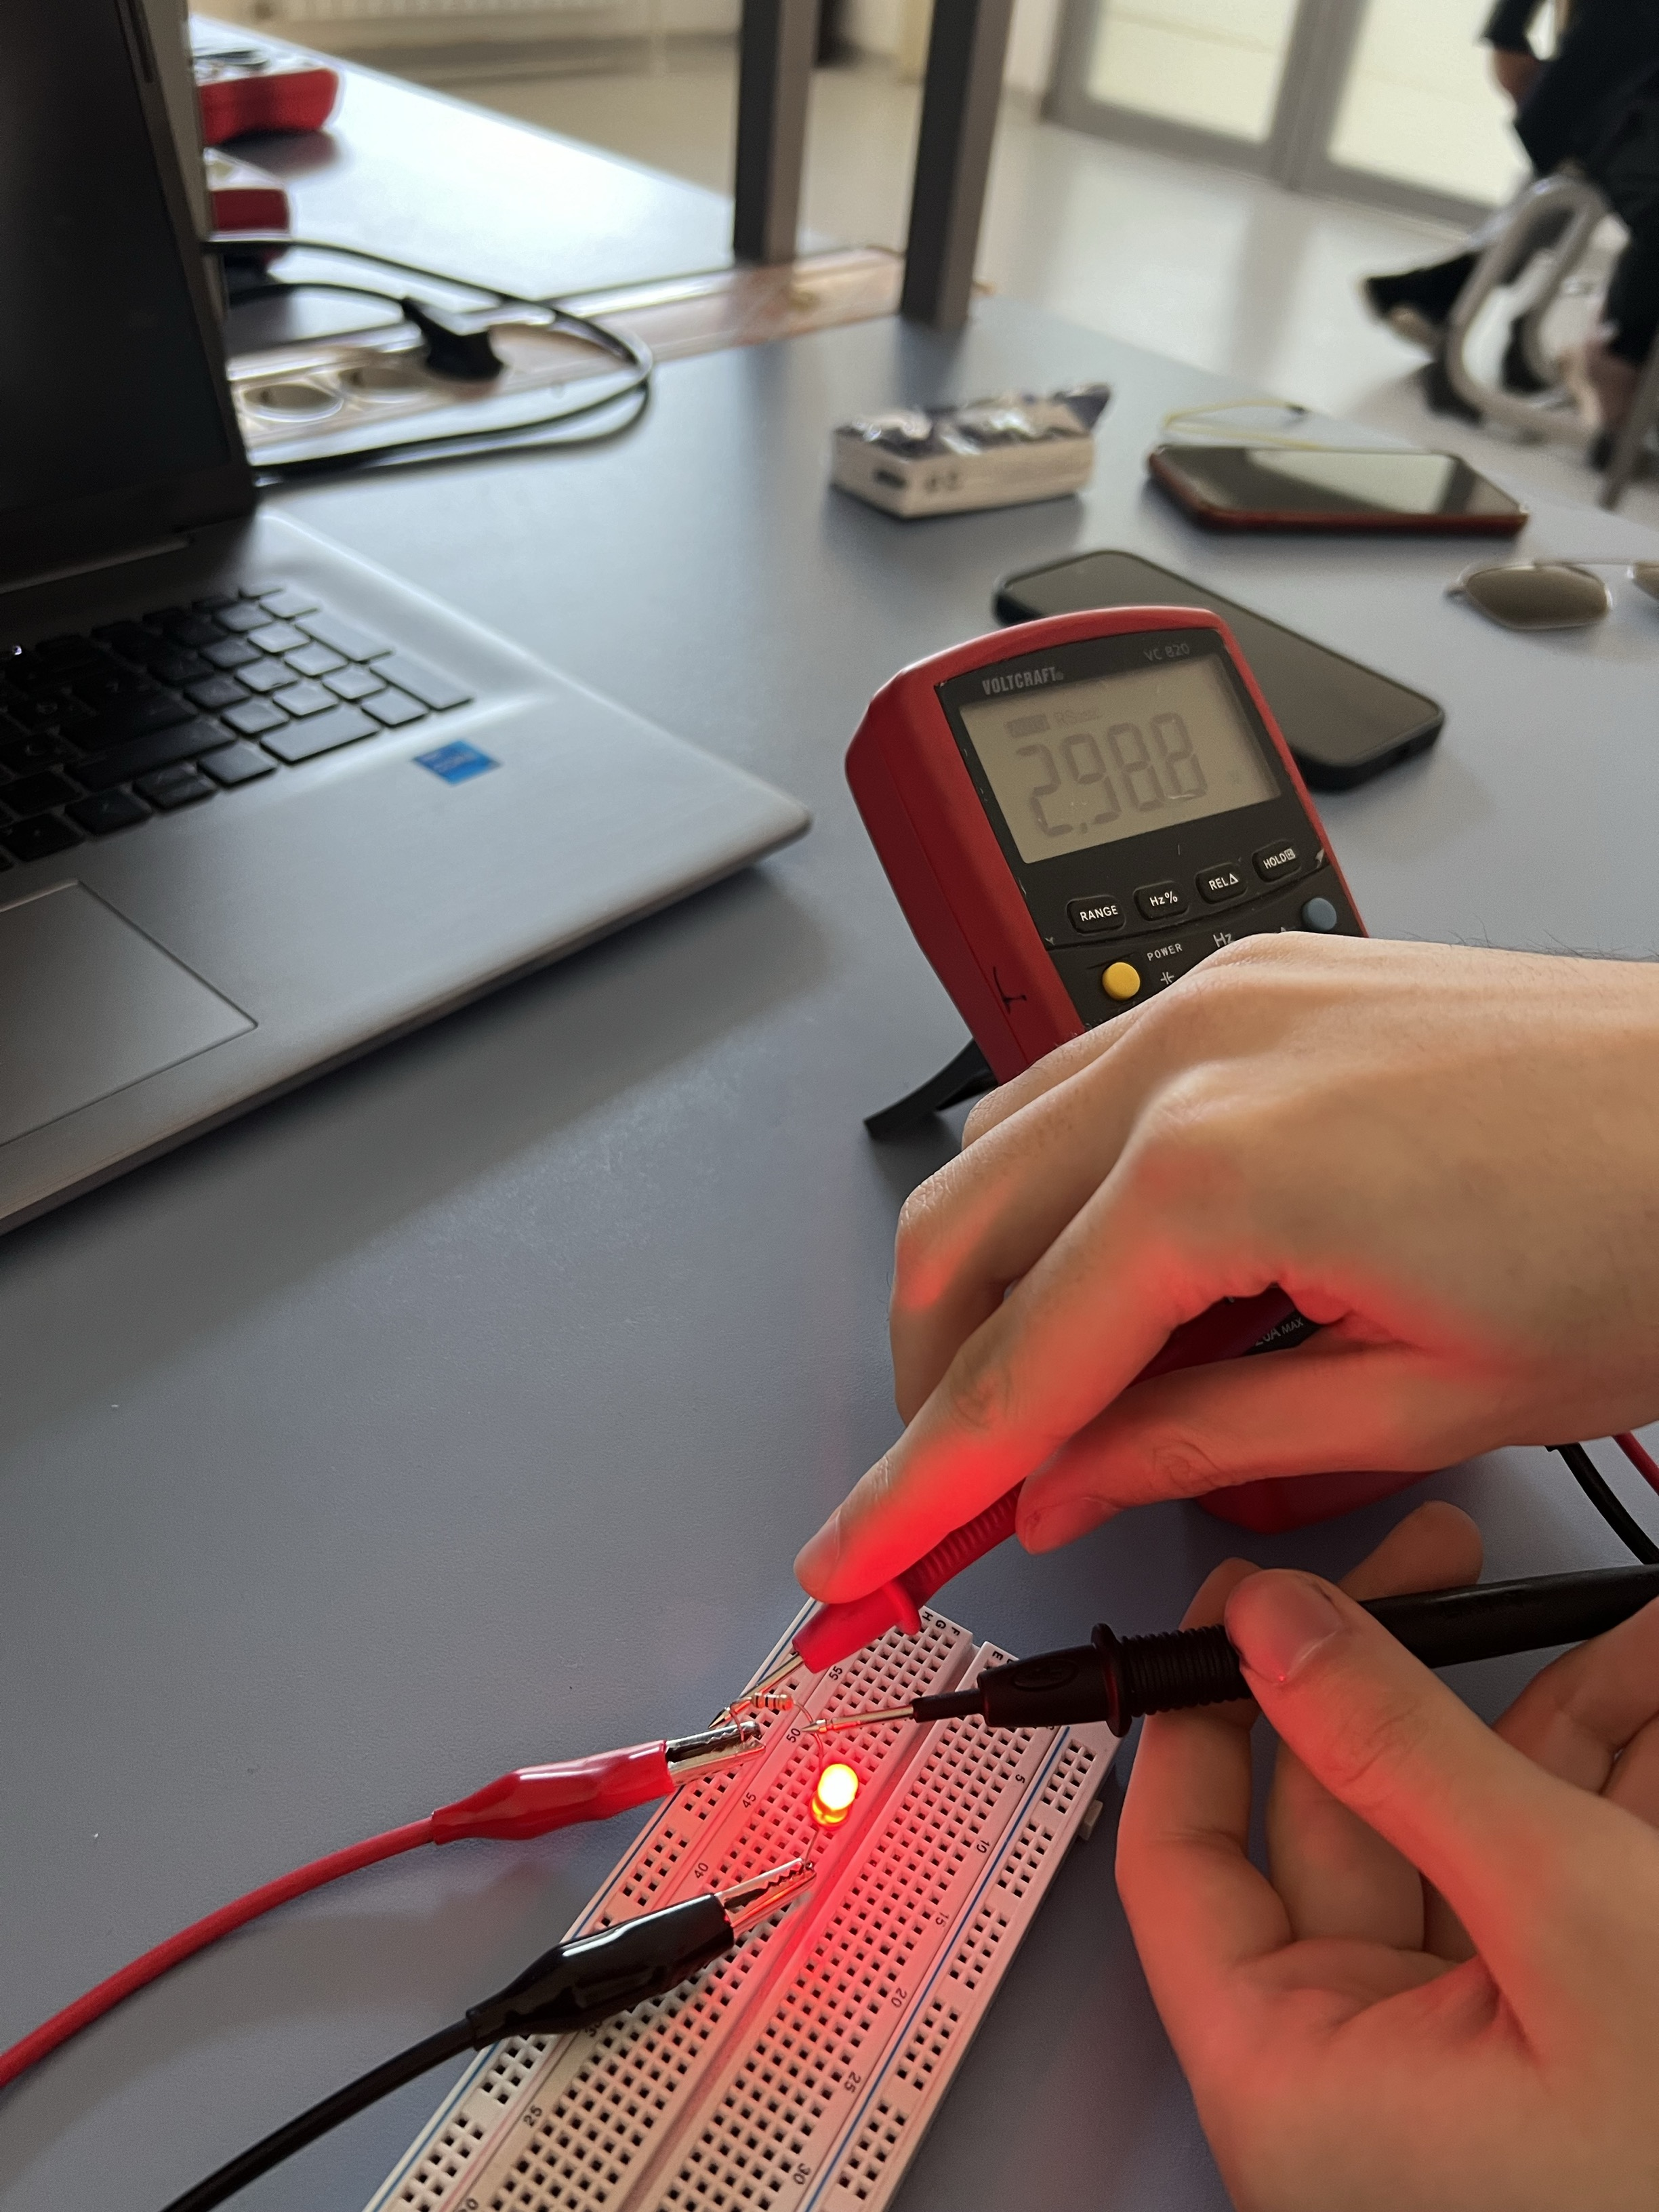
\includegraphics[width=\textwidth]{./images/Circ1_VDrop_Resistor.jpeg}
					\caption{Voltage drop on the resistor}
					\label{sub-fig:VDropResistorCirc1}
				\end{subfigure}
				\caption{Voltage drop across the resistor and the LED}
				\label{fig:circ1VDropResistorAndLED}
			\end{figure}

			As we can see the voltage drop across the resistor and the LED are 2.988V and 2.119V respectively. 
			When we sum these two values we get 5.107V which is equal to the voltage of the power supply.
			One quick note we did say that we were going to set the voltage source to 5V but , as will be shown in Figure \ref{fig:VoltageSourceCirc1},
			the voltage source isn't the most precise

			\begin{table}[h!]
				\centering
				\begin{tabular}{@{}l|S@{}} % l for left, S for siunitx number column
					\toprule
					{Component} & {Voltage Drop (\si{\volt})} \\
					\midrule
					LED & 2.119 \\ \hline
					Resistor & 2.988 \\ \hline
					\textbf{Total} & \textbf{5.107} \\
					\bottomrule
				\end{tabular}
				\caption{Voltage drops across the LED and the resistor}
				\label{tab:circ1VDrops}
			\end{table}

			\pagebreak
			\begin{figure}[h!]
				\centering
				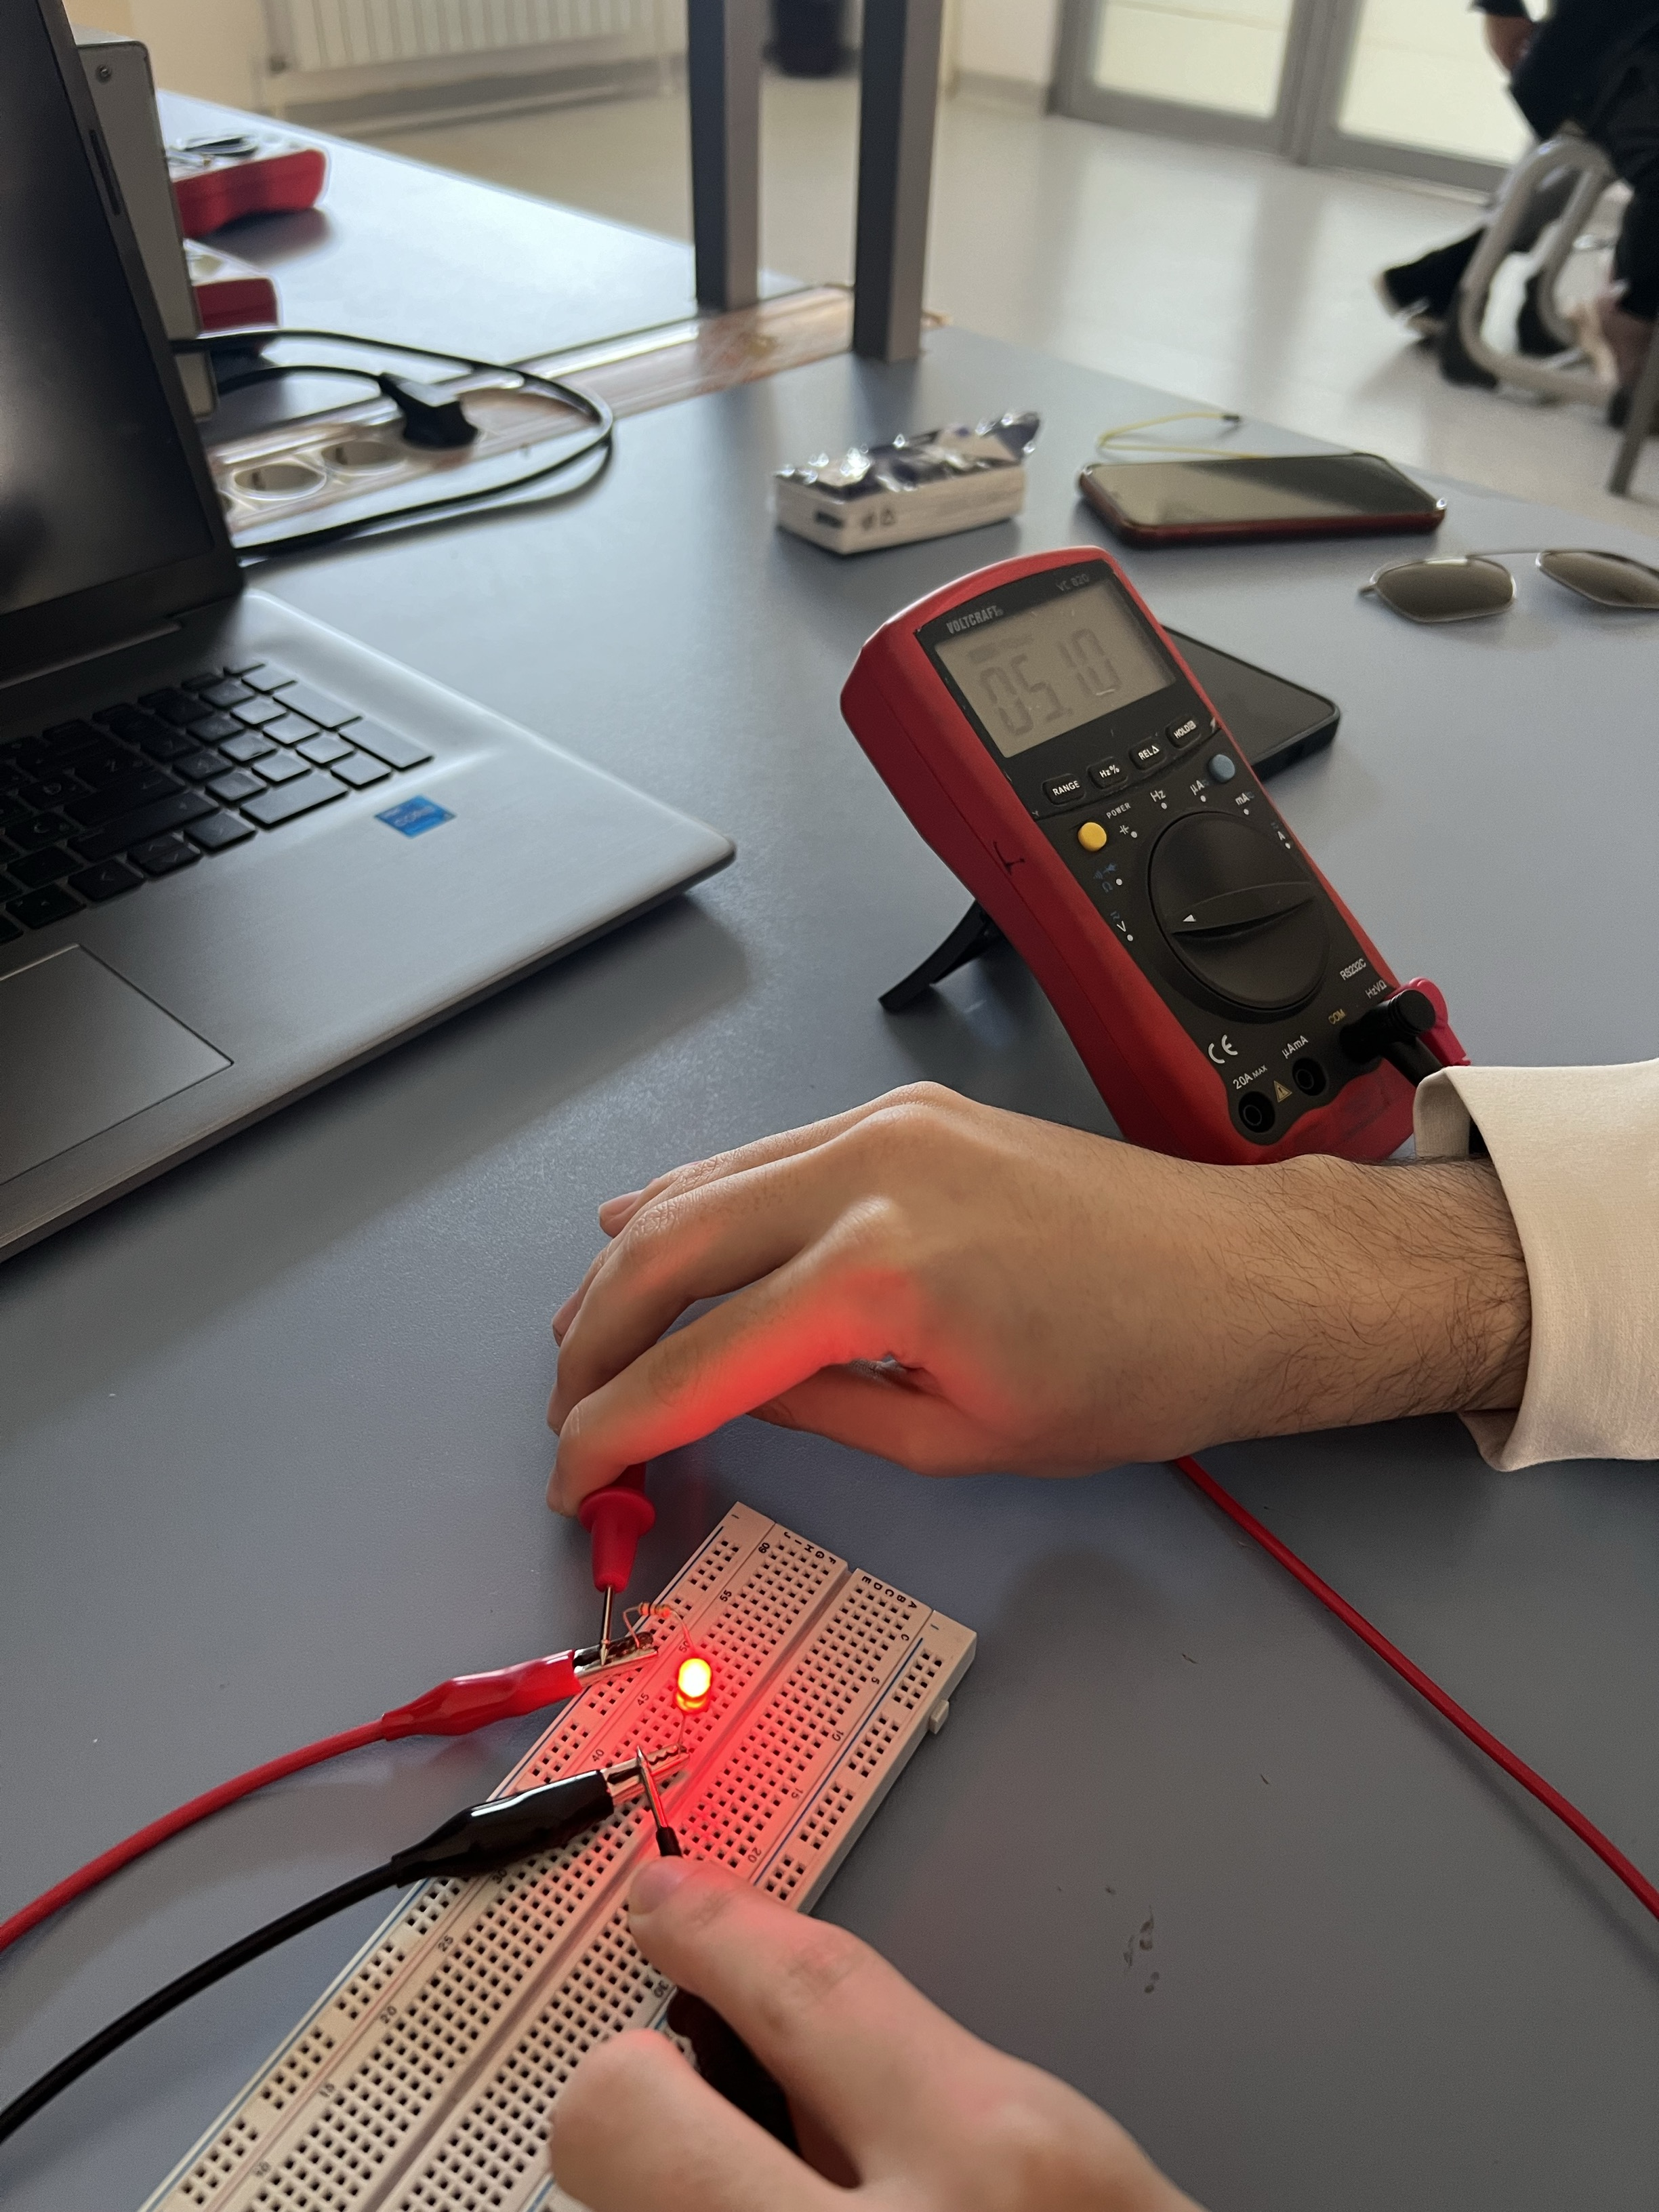
\includegraphics[height = 0.35\textheight]{images/Circ1_VDrop_Circ.jpeg}
				\caption{Voltage of the source}
				\label{fig:VoltageSourceCirc1}
			\end{figure}

			Here as we mentioned before we measured the voltage of the course and got around 5.1V which is close to the 5V that we set it to be.
			Of course this isnt a perfect measurement but it is close enough to show that the voltage source is equal to the sum of the voltage drops across the LED and the resistor,
			hence validating Kirchhoff's Voltage Law.

		\subsection{Changing the voltage source and resistance}
			Since we have already covered this in the previous lab report we will not be covering this in this lab report.
			If you are interested in seeing how the LED behaves when the voltage source is changed or the resistance is changed you can check out the previous lab report.
	
	\pagebreak

	\section{Circuit 2}
		\begin{figure}[h!]
			\centering
			\begin{circuitikz}[scale=0.8, transform shape]
				\draw
				(0,0) to[V, V=\SI{5}{V}] (0,2) -- (2,2) % R10
				(2,2) to[R, l=R3, -*] (2,0)
				(3, 2)to[R, l=R2, -*] (3,0) % R9
				(4,2) to[R, l=R1] (4,0) % R8
				-- (0,0)
				(2, 2) -- (4, 2)
				;
			\end{circuitikz}
			\caption{Circuit with resistors in parallel}
			\label{fig:parallel-resistors}
		\end{figure}

		\subsection{Objectives}
			\begin{itemize}
				\item Make the circuit shown in Figure \ref{fig:parallel-resistors}.
				\item Measure the voltage across each resistor.
			\end{itemize}

		\subsection{Making the circuit}
			To make this circuit we took 3 resistors and connected them in parallel. 
			We then connected the positive terminal of the voltage source to a terminal of the resistors and the negative terminal of the voltage source to the opposite terminal of the resistors.
			You can see the above mentioned circuit on Figure \ref{fig:Physical_Parallel_Circ}

			\begin{figure}[h!]
				\centering
				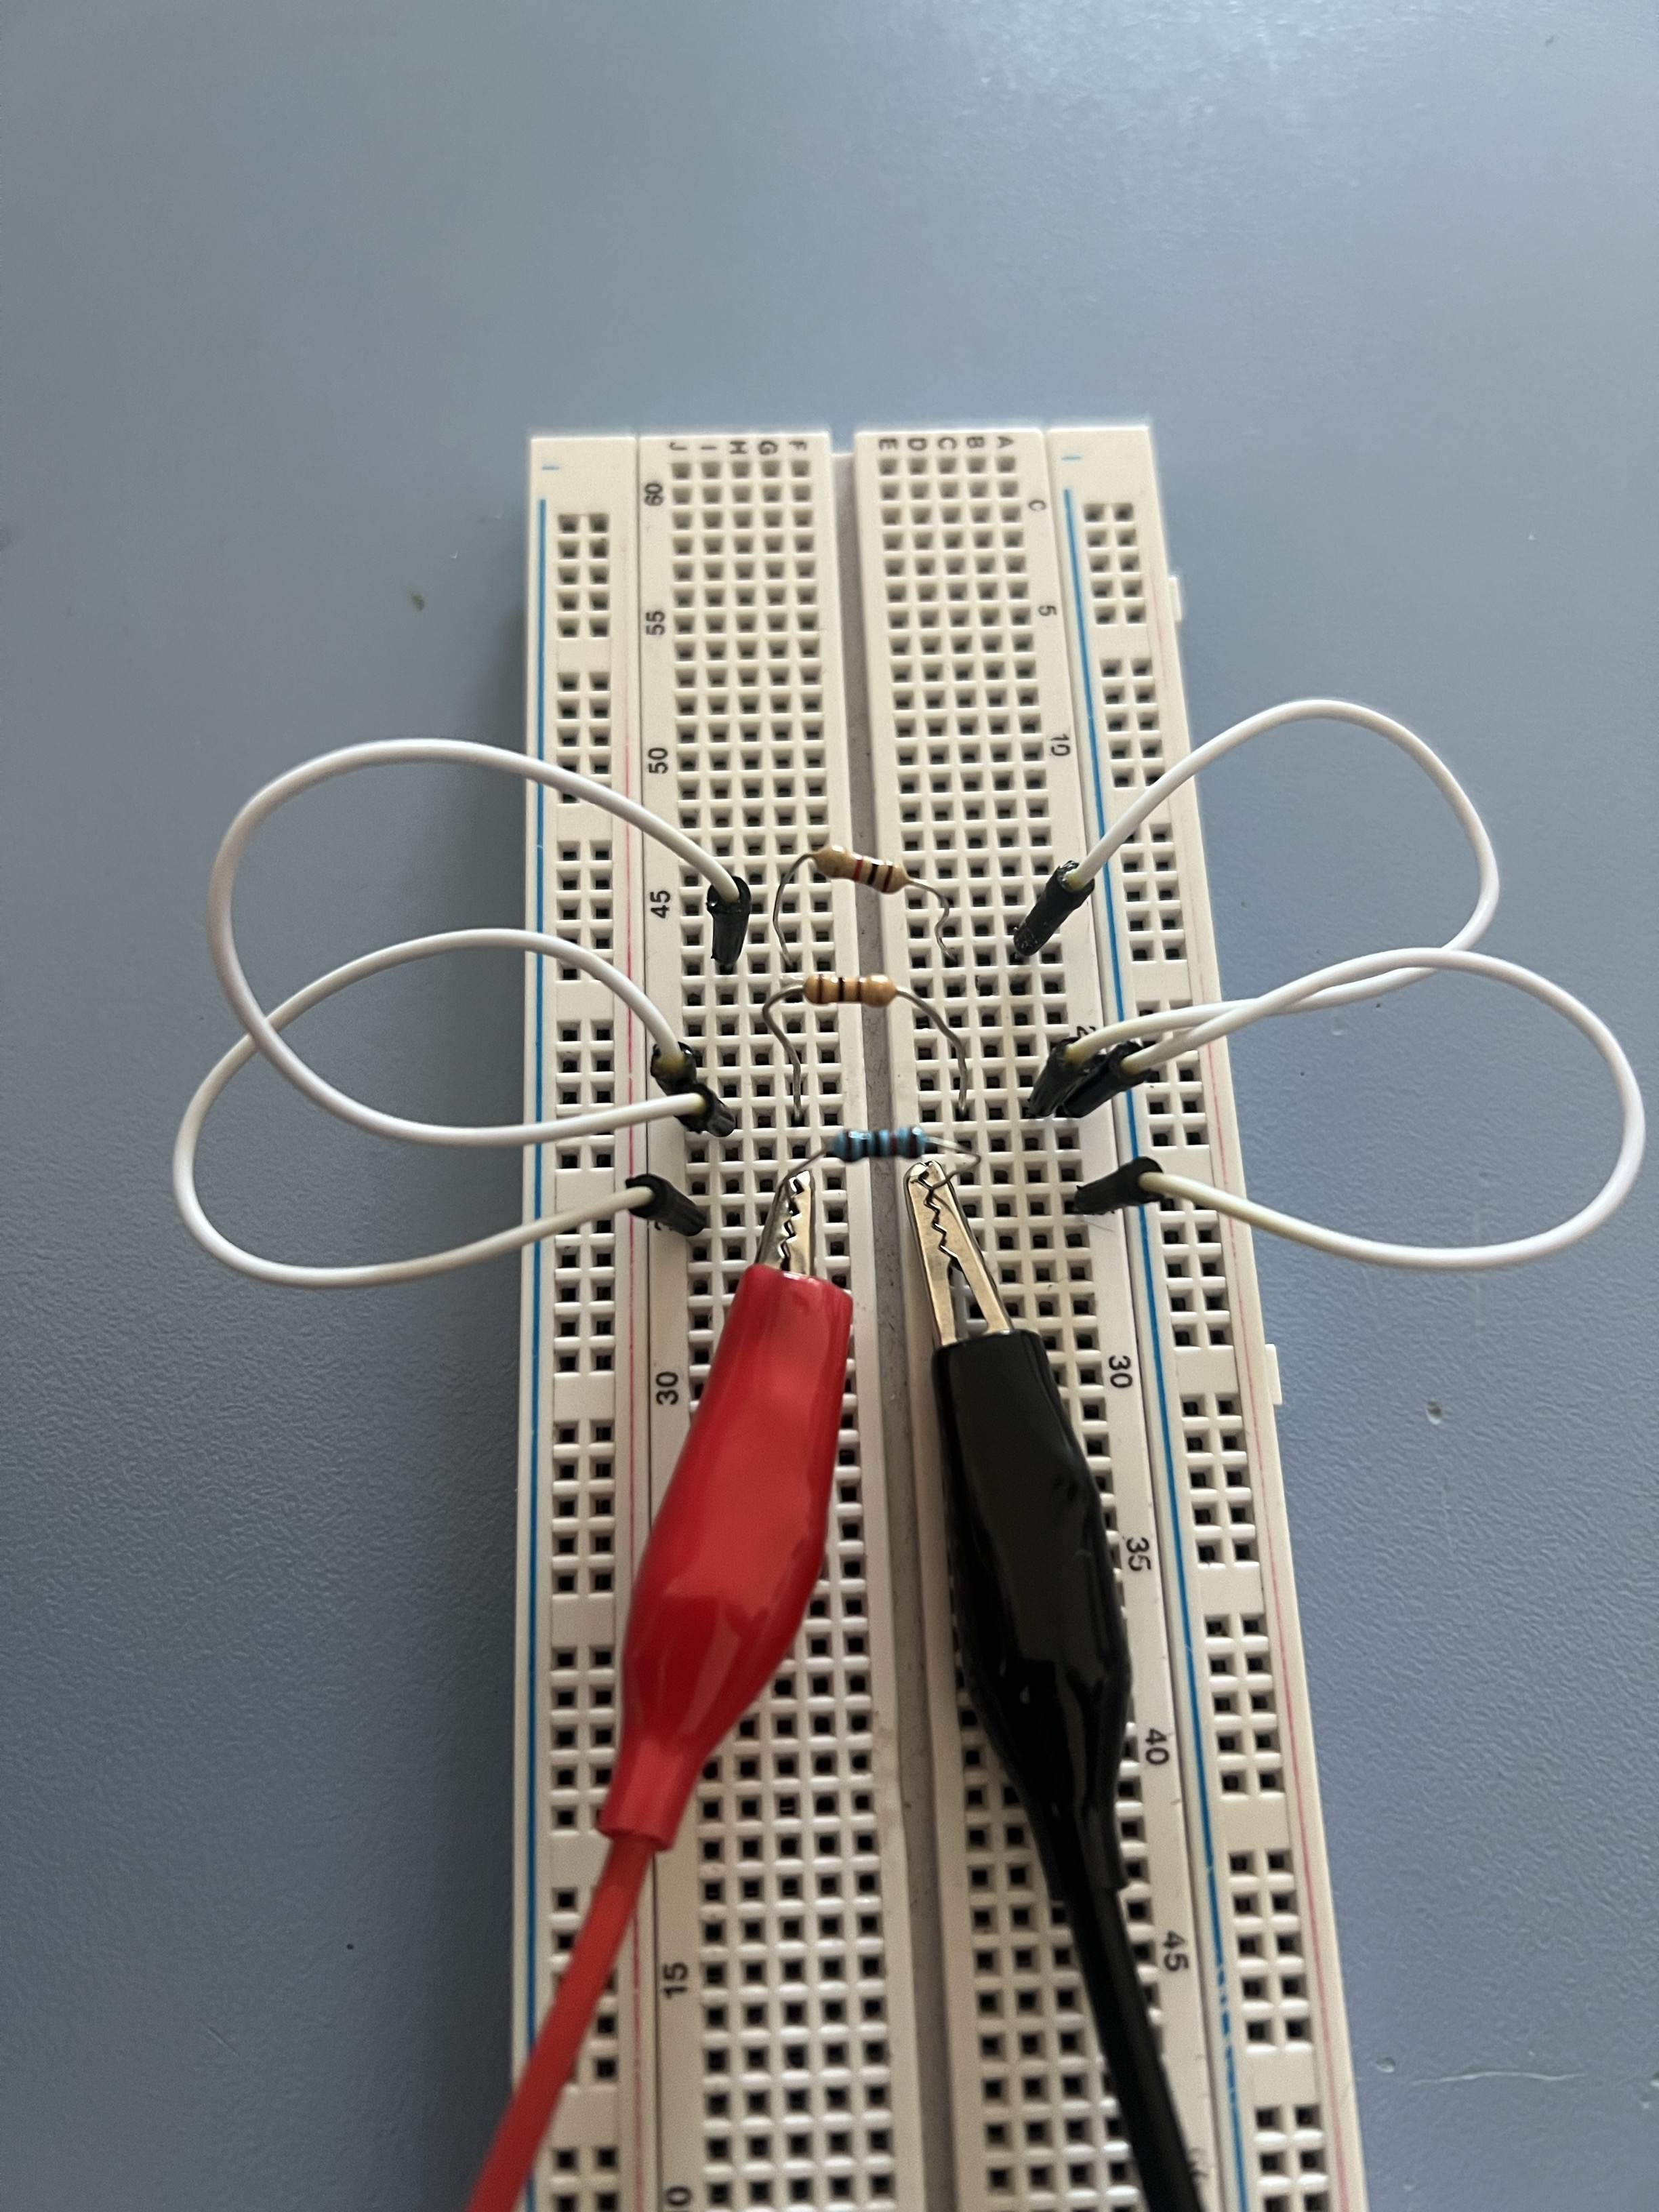
\includegraphics[width = .3\textwidth]{images/Circuit2.jpeg}
				\caption{Parallel resistors circuit made on the breadboard}
				\label{fig:Physical_Parallel_Circ}
			\end{figure}

		
			\pagebreak
		\subsubsection{Measuring the voltage drop on resistor R1}
			To measure the voltage drop across resistor R1, we connected the multimeter in parallel with the resistor and measured the voltage.
			You can see the circuit diagram in Figure \ref{fig:VDropR1Circ2} and the physical setup in Figure \ref{fig:VDropR1Circ2Physical}.

			\begin{figure}[h!]
				\centering
				\begin{circuitikz}[scale=0.8, transform shape]
							\draw
							(0,0) to[V, V=\SI{5}{V}] (0,2) -- (2,2) % R10
							(2,2) to[R, l=R3, -*] (2,0)
							(3, 2)to[R, l=R2, -*] (3,0) % R9
							(4,2) to[R, l=R1] (4,0) % R8
							-- (0,0)
							(2, 2) -- (4, 2)
							(4,2) -- (5.2,2) to[rmeter, t=V] (5.2,0) -- (4,0)  % Voltmeter
							;
					\end{circuitikz}
				\caption{Voltage drop across resistor R1 Diagram}
				\label{fig:VDropR1Circ2}
			\end{figure}

			\begin{figure}[h!]
				\centering
				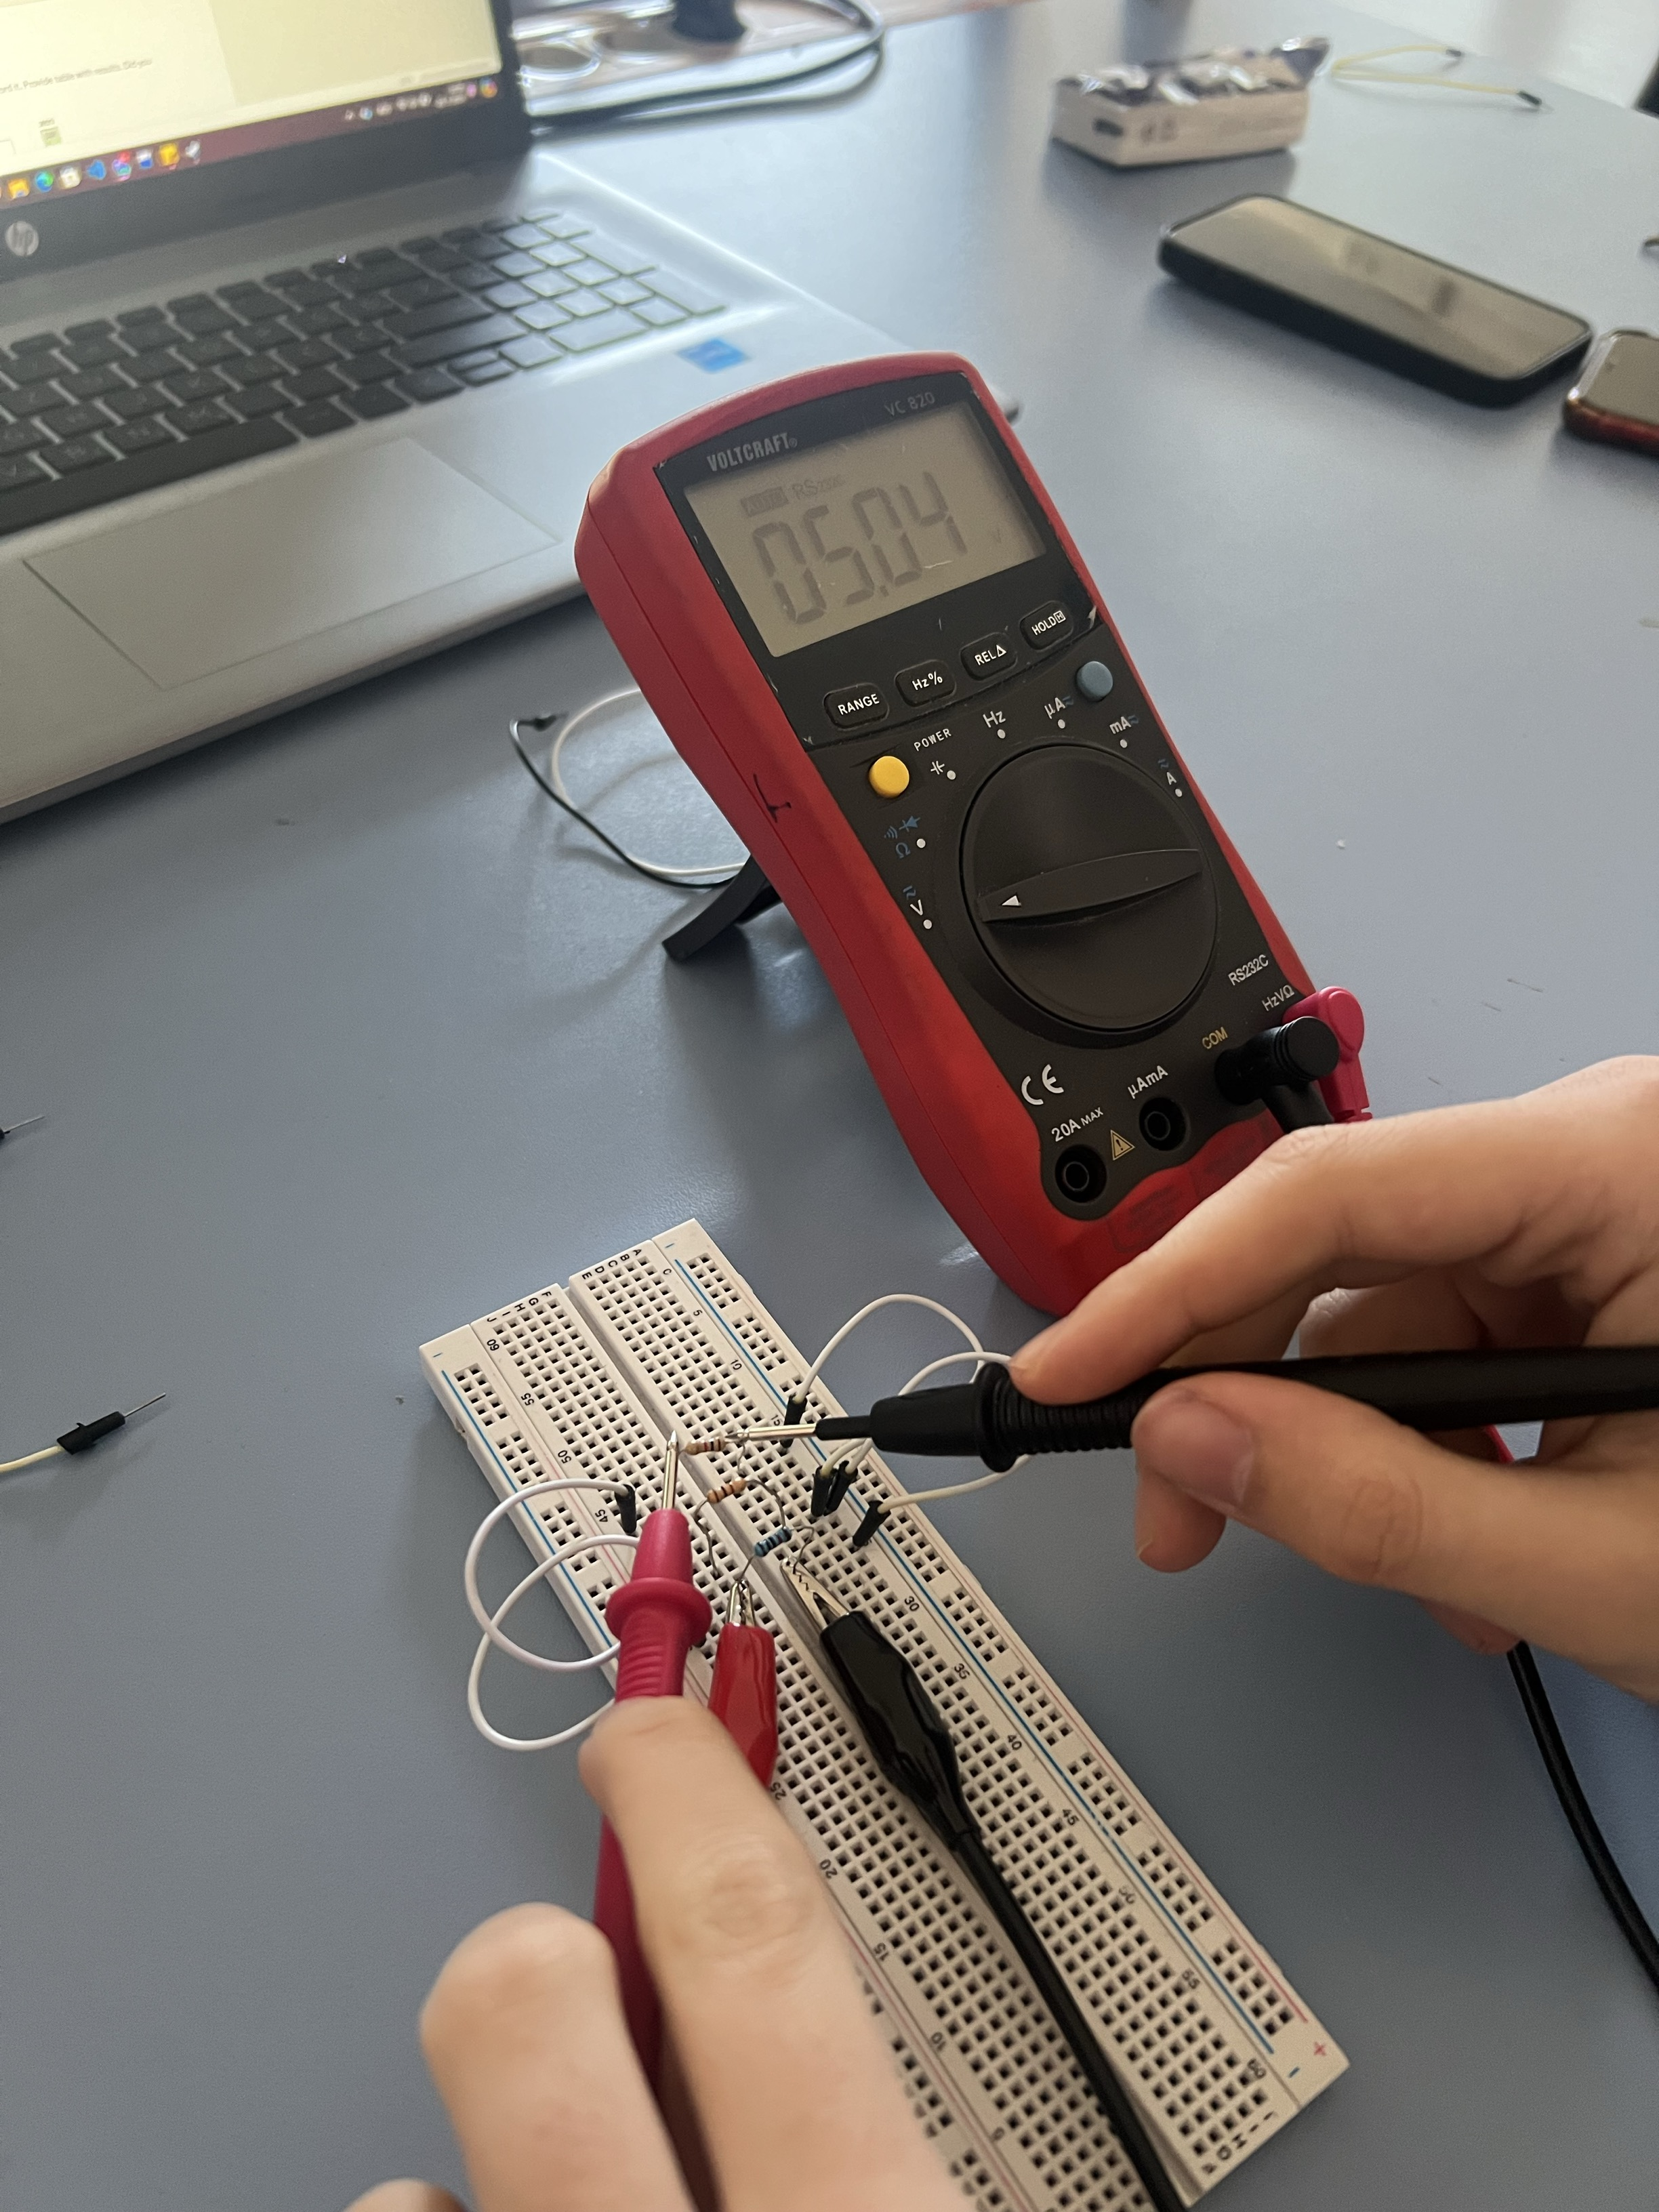
\includegraphics[width = .3\textwidth]{images/MeasuringVDropCirc2.jpeg}
				\caption{Voltage drop across resistor R1}
				\label{fig:VDropR1Circ2Physical}
			\end{figure}

			Since this is a parallel connection the voltage drop on all the resistors should be the same as the voltage of the power source.
		\pagebreak
\end{document}
